%%%%%%%%%%%%%%%%%%%%%%%%%%%%%%%%%%%%%%%%%%%%%%%%%%%%%%%%%%%%%%%%%%%%%%%%%%%%%%%%%%%%%%%%% 
%%%%%%%%%%%%%%%%%%%%%%%%%%%%%%%%%%%%%% Preambule %%%%%%%%%%%%%%%%%%%%%%%%%%%%%%%%%%%%%%%%%
%%%%%%%%%%%%%%%%%%%%%%%%%%%%%%%%%%%%%%%%%%%%%%%%%%%%%%%%%%%%%%%%%%%%%%%%%%%%%%%%%%%%%%%%%%

\documentclass[a4paper, 12pt, leqno]{article}\usepackage[]{graphicx}\usepackage[]{color}
%% maxwidth is the original width if it is less than linewidth
%% otherwise use linewidth (to make sure the graphics do not exceed the margin)
\makeatletter
\def\maxwidth{ %
  \ifdim\Gin@nat@width>\linewidth
    \linewidth
  \else
    \Gin@nat@width
  \fi
}
\makeatother

\definecolor{fgcolor}{rgb}{0.345, 0.345, 0.345}
\newcommand{\hlnum}[1]{\textcolor[rgb]{0.686,0.059,0.569}{#1}}%
\newcommand{\hlstr}[1]{\textcolor[rgb]{0.192,0.494,0.8}{#1}}%
\newcommand{\hlcom}[1]{\textcolor[rgb]{0.678,0.584,0.686}{\textit{#1}}}%
\newcommand{\hlopt}[1]{\textcolor[rgb]{0,0,0}{#1}}%
\newcommand{\hlstd}[1]{\textcolor[rgb]{0.345,0.345,0.345}{#1}}%
\newcommand{\hlkwa}[1]{\textcolor[rgb]{0.161,0.373,0.58}{\textbf{#1}}}%
\newcommand{\hlkwb}[1]{\textcolor[rgb]{0.69,0.353,0.396}{#1}}%
\newcommand{\hlkwc}[1]{\textcolor[rgb]{0.333,0.667,0.333}{#1}}%
\newcommand{\hlkwd}[1]{\textcolor[rgb]{0.737,0.353,0.396}{\textbf{#1}}}%

\usepackage{framed}
\makeatletter
\newenvironment{kframe}{%
 \def\at@end@of@kframe{}%
 \ifinner\ifhmode%
  \def\at@end@of@kframe{\end{minipage}}%
  \begin{minipage}{\columnwidth}%
 \fi\fi%
 \def\FrameCommand##1{\hskip\@totalleftmargin \hskip-\fboxsep
 \colorbox{shadecolor}{##1}\hskip-\fboxsep
     % There is no \\@totalrightmargin, so:
     \hskip-\linewidth \hskip-\@totalleftmargin \hskip\columnwidth}%
 \MakeFramed {\advance\hsize-\width
   \@totalleftmargin\z@ \linewidth\hsize
   \@setminipage}}%
 {\par\unskip\endMakeFramed%
 \at@end@of@kframe}
\makeatother

\definecolor{shadecolor}{rgb}{.97, .97, .97}
\definecolor{messagecolor}{rgb}{0, 0, 0}
\definecolor{warningcolor}{rgb}{1, 0, 1}
\definecolor{errorcolor}{rgb}{1, 0, 0}
\newenvironment{knitrout}{}{} % an empty environment to be redefined in TeX

\usepackage{alltt} %leqno: numéro d'équation à gauche
\pagenumbering{arabic} % choose how to number the pages
\usepackage{a4wide}
%\usepackage[utf8]{inputenc} % accents interprétés
\usepackage{graphicx}
%\usepackage{subfig}
%\usepackage[hmargin=2cm, vmargin = 2cm, noheadfoot]{geometry} %% Pour gérer le format des pages
%\usepackage{layout} %% Pour avoir la longueur des marges
\usepackage[round,sort]{natbib} %% Natbib is a popular style for formatting references.
%\usepackage{multibib}
%\newcites{secnm}{Bibliographie} 
\usepackage{verbatim} % for multiline comments
\usepackage{amssymb} %symbole de maths
\usepackage{amsmath} %idem
%\usepackage{stmaryrd} %% Symbole flèche à l'envers
\usepackage{amsfonts}
\usepackage[english]{babel} %% Les titres en anglais
\usepackage[utf8]{inputenc} % accents interprétés
\usepackage{array} %% Pour centrer verticalement le contenu d'un tableau, entre autres...
\setcounter{secnumdepth}{4} %% Profondeur des sections, subsections
\usepackage{setspace} %% Gère l'interligne: singlespacing, doublespacing
\singlespacing
\usepackage[colorlinks=true,citecolor=blue]{hyperref} %% Gère les hyperliens
%\usepackage{textcomp} %% Symbole pourmille
\usepackage{lineno} %% Numérotation des lignes
\usepackage{longtable}
\setlength{\LTleft}{-5cm plus 1 fill}
\setlength{\LTright}{-5cm plus 1 fill}
\usepackage{booktabs}
%\usepackage{colortabs} % can't be found
\usepackage{xcolor}
\usepackage{colortbl} %% color text and table rows
%\usepackage{arydshln} %% dashlines for tabular
%\usepackage{sidecap}
\newcommand{\logit}{\text{logit}}
\newcommand{\bs}[1]{\boldsymbol{#1}}
\newcommand{\p}{\text{p}}
% For changes in tables
\newcommand{\SetRowColor}[1]{\noalign{\gdef\RowColorName{#1}}\rowcolor{\RowColorName}}
\definecolor{gray90}{gray}{0.9}
\newcommand{\mymulticolumn}[3]{\multicolumn{#1}{>{\columncolor{gray90}}#2}{#3}}
\newcommand{\sizeBigTable}{\fontsize{9pt}{9pt}\selectfont}

\newcolumntype{L}[1]{>{\raggedright\let\newline\\\arraybackslash\hspace{0pt}}p{#1}}
\newcolumntype{C}[1]{>{\centering\let\newline\\\arraybackslash\hspace{0pt}}p{#1}}
\newcolumntype{R}[1]{>{\raggedleft\let\newline\\\arraybackslash\hspace{0pt}}p{#1}}

%%%%%%%%%%%%%%%%%%%%%%%%%%%%%%%%%%%%%%%%%%%%%%%%%%%%%%%%%%%%%%%%%%%%%%%%%%%%%%%%%%%%%%%%%%
%%%%%%%%%%%%%%%%%%%%%%%%%%%%%%%%%%%%%% Title %%%%%%%%%%%%%%%%%%%%%%%%%%%%%%%%%%%%%%%%%%%%%
%%%%%%%%%%%%%%%%%%%%%%%%%%%%%%%%%%%%%%%%%%%%%%%%%%%%%%%%%%%%%%%%%%%%%%%%%%%%%%%%%%%%%%%%%%

\title{Hierarchical Bayesian species distribution models with the \textbf{hSDM} R Package}
\date{}
\author{}

%%%%%%%%%%%%%%%%%%%%%%%%%%%%%%%%%%%%%%%%%%%%%%%%%%%%%%%%%%%%%%%%%%%%%%%%%%%%%%%%%%%%%%%%%%
%%%%%%%%%%%%%%%%%%%%%%%%%%%%%%%%%%%%%% Knitr %%%%%%%%%%%%%%%%%%%%%%%%%%%%%%%%%%%%%%%%%%%%%
%%%%%%%%%%%%%%%%%%%%%%%%%%%%%%%%%%%%%%%%%%%%%%%%%%%%%%%%%%%%%%%%%%%%%%%%%%%%%%%%%%%%%%%%%%

%\VignetteEngine{knitr::knitr}
%\VignetteIndexEntry{User manual for hSDM R package}

%%%%%%%%%%%%%%%%%%%%%%%%%%%%%%%%%%%%%%%%%%%%%%%%%%%%%%%%%%%%%%%%%%%%%%%%%%%%%%%%%%%%%%%%%%
%%%%%%%%%%%%%%%%%%%%%%%%%%%%%%%%%%%%%% Document %%%%%%%%%%%%%%%%%%%%%%%%%%%%%%%%%%%%%%%%%%
%%%%%%%%%%%%%%%%%%%%%%%%%%%%%%%%%%%%%%%%%%%%%%%%%%%%%%%%%%%%%%%%%%%%%%%%%%%%%%%%%%%%%%%%%%
\IfFileExists{upquote.sty}{\usepackage{upquote}}{}

\begin{document}
\maketitle
\vspace{-1cm}
\begin{center}
  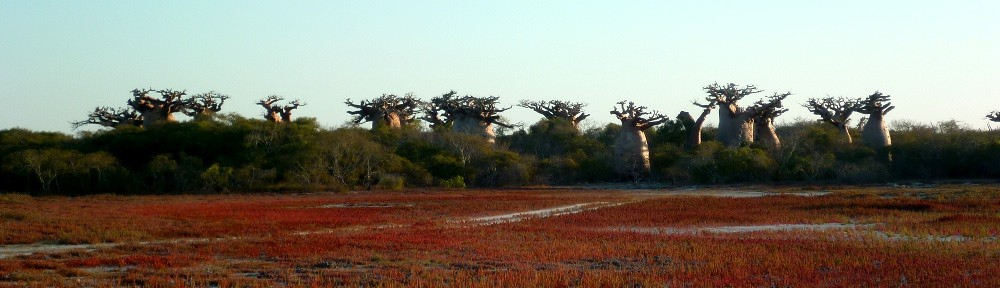
\includegraphics[width=\textwidth]{header.jpg}\\
  \textit{Adansonia grandidieri} Baill. next to Andavadoaka village (southwest Madagascar).
\end{center}
\vspace{1cm}
\begin{center}
  \large{Ghislain Vieilledent$^{\star,1}$}
\end{center}

\vspace{0.3cm}

%% {\footnotesize
%% \begin{flushleft}
%%   \textbf{Type of article:} Data paper for \textit{Annals of Forest Science}\\
%%   \textbf{Thematic issue:} GlobAllomeTree web platform\\
%%   \textbf{Running title:} Cirad wood density data base\\
%%   \textbf{Number of words and objects:} whole manuscript (X words) with abstract (X words),
%%   main text (X words), references (X, X words), table and figure legends (X, X words)\\
%% \end{flushleft}}

%\vspace{0.2cm}

{\footnotesize
  \begin{flushleft}
    $[\star]$ \textbf{Corresponding author:}
    \textbackslash{E-mail}:~ghislain.vieilledent@cirad.fr
    \textbackslash{Phone}:~+33.(0)4.67.59.37.51
    \textbackslash{Fax}:~+33.(0)4.67.59.39.09\\
    $[1]$ \textbf{Cirad} -- UPR BSEF, F–34398 Montpellier, France\\
\end{flushleft}}

\newpage
%\doublespacing
%\linenumbers

\renewcommand{\abstractname}{Abstract}
\newcommand{\keywords}[1]{\par\noindent
{\small{\em Keywords\/}: #1}}

\begin{abstract}

  Work in progess...
  
  \vspace{0.5cm}

  \keywords{R}

\end{abstract}

\newpage

%%=============================
%% Change default shunk options



\section{Introduction}

\section{Species distribution models}

\subsection{Binomial model}
\label{sec:binomial}

\subsubsection{Mathematical formulation}

Let's consider a random variable $y_{i(jt)}$ (abbreviated $y_i$) representing the total
number of presences of a species after several visits $v_{i(jt)}$ (abbreviated $v_i$) at a
particular site $j$ at time $t$ ($t$ can indicate a day, a year, etc. thus allowing
several visits at time $t$). Random variable $y_i$ can take values from 0 to $v_i$ and can
be assumed to follow a Binomial distribution having parameters $v_i$ and $\theta_{i(jt)}$
(Eq.~\ref{eq:binomial}). $\theta_{i(jt)}$ (abbreviated $\theta_i$) can be interpreted as
the probability of presence of the species at site $j$ and time $t$. Using a logit link
function, $\theta_i$ can be expressed as a linear model combining explicative variables
$X_{i(jt)}$ and parameters $\beta$ (Eq.~\ref{eq:binomial}).

\begin{equation}
  \begin{tabular}{c}
    $y_i \sim \mathcal{B}inomial(v_i,\theta_i)$ \\
    ~ \\
    $\logit(\theta_i) = X_{i(jt)} \beta$ \\
  \end{tabular}
  \label{eq:binomial}
\end{equation}

Using this statistical model, we aim at representing a ``suitability process''. Given
environmental variables $X_{i(jt)}$, how much is habitat at site $j$ and at time $t$
suitable for the species under consideration? Parameters $\beta$ indicate how much each
environmental variable contributes to the suitability process. Like every other function
in the \textbf{hSDM} R package, function \texttt{hSDM.binomial()} estimates the parameters
$\beta$ of such a model in a Bayesian framework. Parameter inference is done using a Gibbs
sampler including a Metropolis algorithm. The Gibbs sampler is coded in the C language to
optimize computation efficiency.

\subsubsection{Data generation}

To explore the characteristics of the \texttt{hSDM.binomial()} function, we can generate a
virtual data-set on the basis of the Binomial model described above
(Eq.~\ref{eq:binomial}). In the most general case (presence/absence data or
presence/pseudo-absence data), a site $j$ is visited once at time $t$ and $v_i=1$. Thus,
the random variable $y_i$ follows a Bernoulli distribution having parameters $\theta_i$
and habitat characteristics $X_{i(jt)}$ are fixed for site $j$. We will generate a virtual
data-set in this particular case. For data generation, we can import virtual altitudinal
data in R. Altitude will be used as an explicative variable to determine habitat
suitability, i.e. the probability of presence of a virtual species. Altitudinal data are
available on the website of the \textbf{hSDM} R package hosted on Sourceforge
(\url{http://hsdm.sourceforge.net/altitude.csv}).

These data can be transformed into a raster using function \texttt{rasterFromXYZ()} from
the \textbf{raster} package. The raster has 2500 cells (50 columns and 50 rows) and the
altitude is comprised roughly between 100 and 600~m (Fig.~\ref{fig:Altitude}). For linear
models, explicative variables are usually centered and scaled to facilitate inference and
interpretation of model parameters.

\begin{knitrout}\small
\definecolor{shadecolor}{rgb}{0.969, 0.969, 0.969}\color{fgcolor}\begin{kframe}
\begin{alltt}
\hlcom{# Import altitudinal data}
\hlkwd{require}\hlstd{(raster)}
\hlstd{fname} \hlkwb{<-} \hlstr{"http://hsdm.sourceforge.net/altitude.csv"}
\hlstd{alt.df} \hlkwb{<-} \hlkwd{read.csv}\hlstd{(fname,}\hlkwc{header}\hlstd{=}\hlnum{TRUE}\hlstd{)}
\hlstd{alt.orig} \hlkwb{<-} \hlkwd{rasterFromXYZ}\hlstd{(alt.df)}
\hlkwd{plot}\hlstd{(alt.orig)}
\hlcom{# Center and scale altitudinal data}
\hlstd{alt} \hlkwb{<-} \hlkwd{scale}\hlstd{(alt.orig,}\hlkwc{center}\hlstd{=}\hlnum{TRUE}\hlstd{,}\hlkwc{scale}\hlstd{=}\hlnum{TRUE}\hlstd{)}
\hlkwd{plot}\hlstd{(alt)}
\end{alltt}
\end{kframe}
\end{knitrout}


\begin{figure}[!h] 
  \begin{tabular}{cc}
    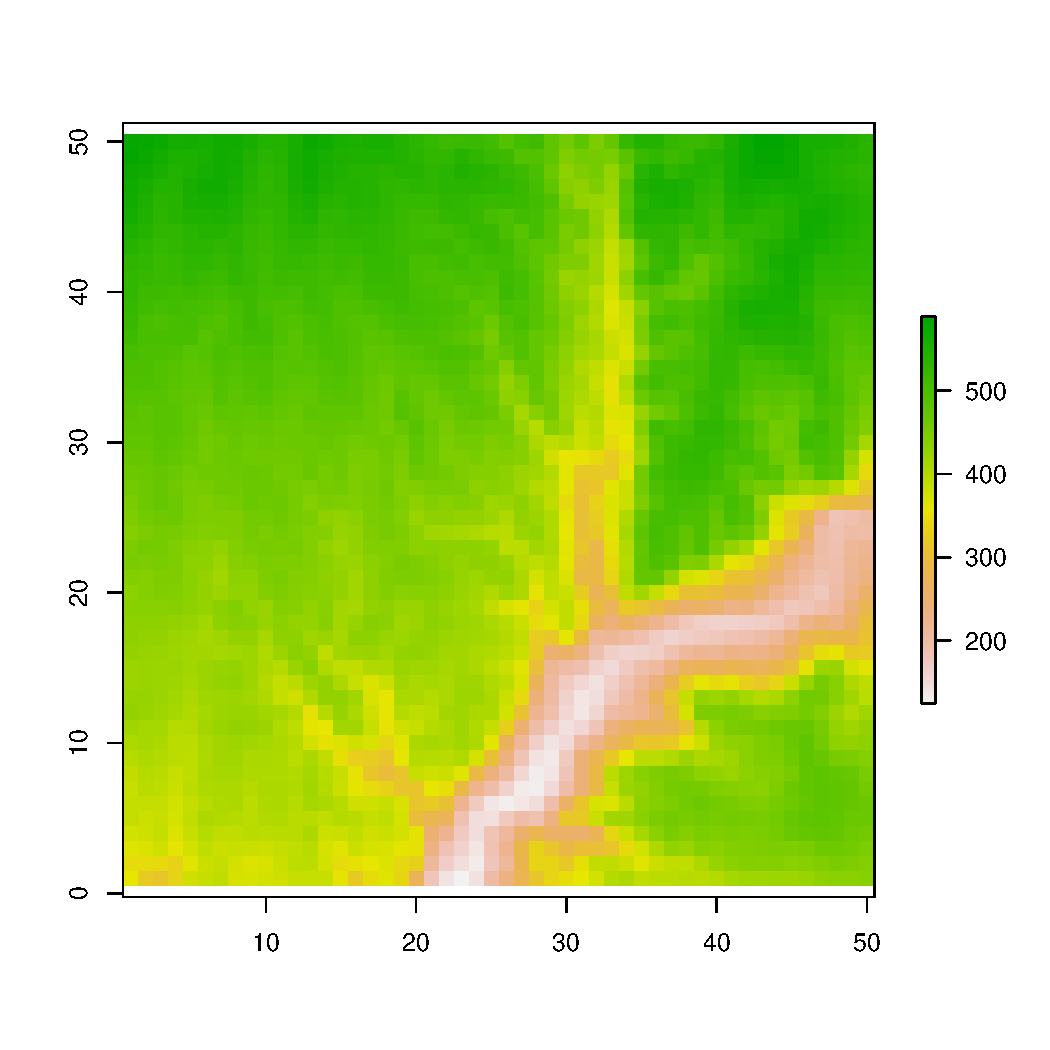
\includegraphics[width=8cm]{figures/Altitude1.pdf} &
    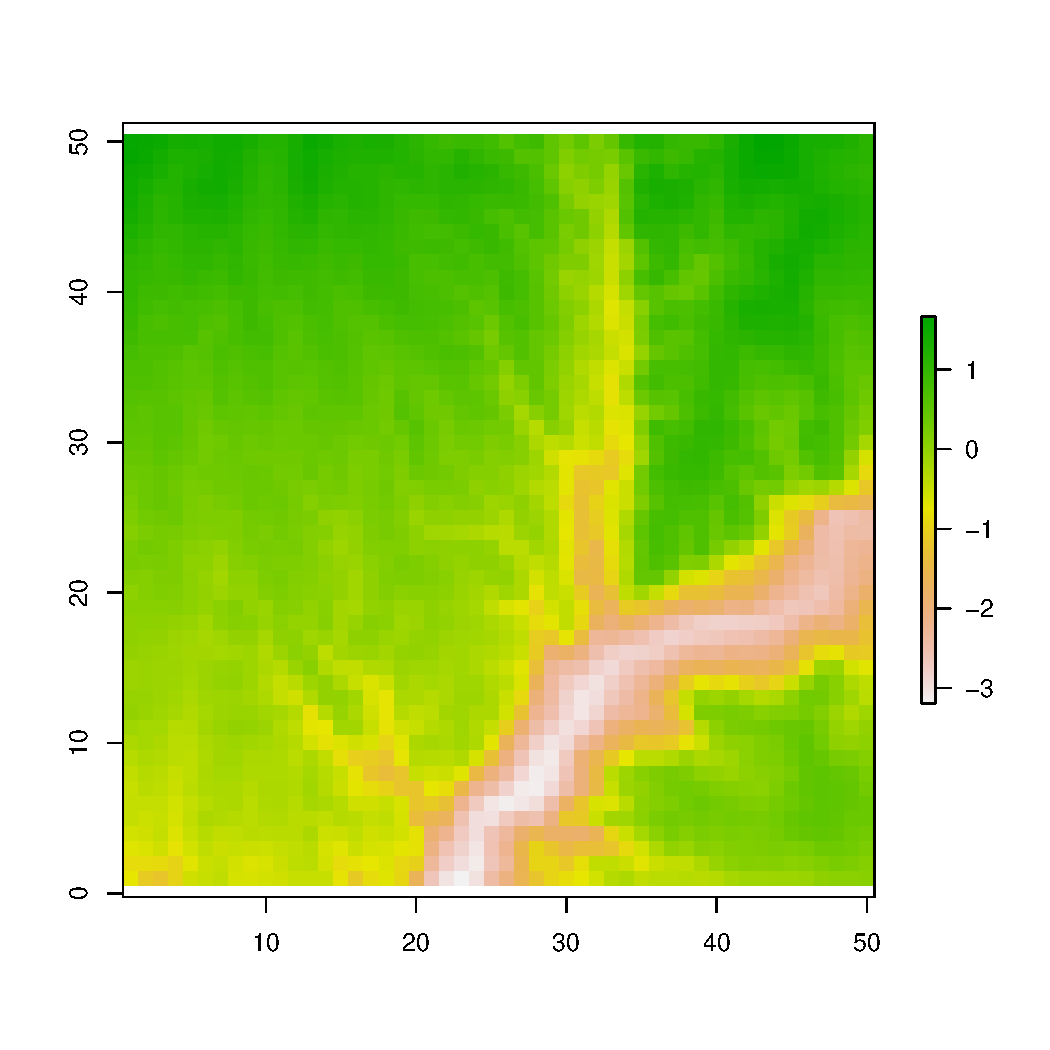
\includegraphics[width=8cm]{figures/Altitude2.pdf} \\
  \end{tabular}
  \caption{\textbf{Altitudinal data}. Original values (in m) on the left. Centered and
    scaled values on the right.}
  \label{fig:Altitude}
\end{figure}

A quadratic effect of the altitude (variable denoted $x$) is used to compute the
probability of presence of the species (Eq.~\ref{eq:bernoulli}).

\begin{equation}
  \begin{tabular}{c}
    $y_i \sim \mathcal{B}ernoulli(\theta_i)$ \\
    ~ \\
    $\logit(\theta_i) = \beta_0 + \beta_1 x_i + \beta_2 x_i^2$ \\
  \end{tabular}
  \label{eq:bernoulli}
\end{equation}

We fix the parameters to $\beta_0=1$, $\beta_1=2$ and $\beta_2=-4$. The species has a
higher probability of presence at intermediate altitudinal values
(Fig.~\ref{fig:theta-binomial}).

\begin{knitrout}\small
\definecolor{shadecolor}{rgb}{0.969, 0.969, 0.969}\color{fgcolor}\begin{kframe}
\begin{alltt}
\hlcom{# Load hSDM library}
\hlkwd{library}\hlstd{(hSDM)}
\hlcom{# Target parameters}
\hlstd{beta.target} \hlkwb{<-} \hlkwd{matrix}\hlstd{(}\hlkwd{c}\hlstd{(}\hlnum{1}\hlstd{,}\hlnum{2}\hlstd{,}\hlopt{-}\hlnum{4}\hlstd{),}\hlkwc{ncol}\hlstd{=}\hlnum{1}\hlstd{)}
\hlcom{# Matrix of covariates (including the intercept)}
\hlstd{X} \hlkwb{<-} \hlkwd{cbind}\hlstd{(}\hlkwd{rep}\hlstd{(}\hlnum{1}\hlstd{,}\hlkwd{ncell}\hlstd{(alt)),}\hlkwd{values}\hlstd{(alt),(}\hlkwd{values}\hlstd{(alt))}\hlopt{^}\hlnum{2}\hlstd{)}
\hlcom{# Probability of presence as a quadratic function of altitude}
\hlstd{logit.theta} \hlkwb{<-} \hlstd{X} \hlopt \hlstd{beta.target}
\hlstd{theta} \hlkwb{<-} \hlkwd{inv.logit}\hlstd{(logit.theta)}
\hlcom{# Transform the probability of presence into a raster}
\hlstd{theta} \hlkwb{<-} \hlkwd{rasterFromXYZ}\hlstd{(}\hlkwd{cbind}\hlstd{(}\hlkwd{coordinates}\hlstd{(alt),theta))}
\hlcom{# Plot the probability of presence}
\hlcom{## require(fields)}
\hlcom{## col.prob <- colorRampPalette(c("transparent","blue","green",}
\hlcom{##                                "yellow","orange","red","brown"))}
\hlcom{## plot(theta,col=col.prob(255))}
\hlkwd{plot}\hlstd{(theta,}\hlkwc{col}\hlstd{=}\hlkwd{rev}\hlstd{(}\hlkwd{heat.colors}\hlstd{(}\hlnum{255}\hlstd{)))}
\end{alltt}
\end{kframe}
\end{knitrout}


\begin{figure}[!h] 
  \centering 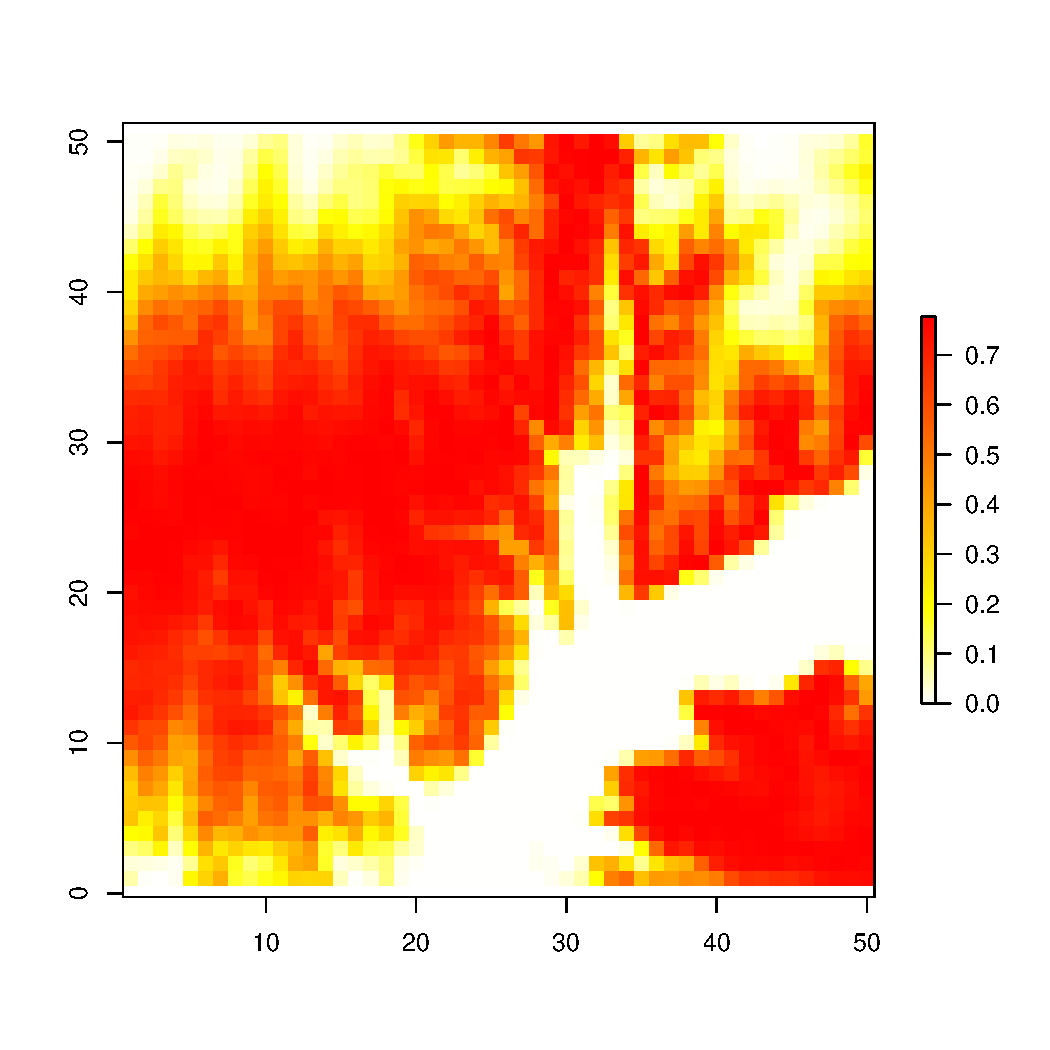
\includegraphics[width=8cm]{figures/theta-binomial.pdf}
  \caption{\textbf{Probability of presence}.}
  \label{fig:theta-binomial}
\end{figure}

We can assume a number $n$ of points in the landscape where we have been able to observe
or not the presence of the species. We can simulate the presence or absence of the species
at these $n$ points given our model (Fig.~\ref{fig:observations-binomial}).

\begin{knitrout}\small
\definecolor{shadecolor}{rgb}{0.969, 0.969, 0.969}\color{fgcolor}\begin{kframe}
\begin{alltt}
\hlcom{# Load dismo library}
\hlkwd{require}\hlstd{(dismo)} \hlcom{# For randomPoints() function}
\hlcom{# Number of observation points}
\hlstd{nobspt} \hlkwb{<-} \hlnum{200}
\hlcom{# Set seed for repeatability}
\hlstd{seed} \hlkwb{<-} \hlnum{1234}
\hlcom{# Sample the observations in the landscape}
\hlkwd{set.seed}\hlstd{(seed)}
\hlstd{obs} \hlkwb{<-} \hlkwd{randomPoints}\hlstd{(alt,nobspt)}
\hlcom{# Extract altitude data for observations}
\hlstd{alt.obs} \hlkwb{<-} \hlkwd{extract}\hlstd{(alt,obs)}
\hlcom{# Compute theta for these observations}
\hlstd{X} \hlkwb{<-} \hlkwd{cbind}\hlstd{(}\hlkwd{rep}\hlstd{(}\hlnum{1}\hlstd{,nobspt),alt.obs,alt.obs}\hlopt{^}\hlnum{2}\hlstd{)}
\hlstd{logit.theta.obs} \hlkwb{<-} \hlstd{X} \hlopt \hlstd{beta.target}
\hlstd{theta.obs} \hlkwb{<-} \hlkwd{inv.logit}\hlstd{(logit.theta.obs)}
\hlcom{# Simulate observations}
\hlstd{trials} \hlkwb{<-} \hlkwd{rep}\hlstd{(}\hlnum{1}\hlstd{,nobspt)}
\hlkwd{set.seed}\hlstd{(seed)}
\hlstd{Y} \hlkwb{<-} \hlkwd{rbinom}\hlstd{(nobspt,trials,theta.obs)}
\hlcom{# Group explicative and response variables in a data-frame}
\hlstd{data.obs.df} \hlkwb{<-} \hlkwd{data.frame}\hlstd{(Y,trials,}\hlkwc{alt}\hlstd{=X[,}\hlnum{2}\hlstd{],}\hlkwc{alt2}\hlstd{=X[,}\hlnum{3}\hlstd{])}
\hlcom{# Transform observations in a spatial object}
\hlkwd{require}\hlstd{(sp)}
\hlstd{data.obs} \hlkwb{<-} \hlkwd{SpatialPointsDataFrame}\hlstd{(}\hlkwc{coords}\hlstd{=}\hlkwd{coordinates}\hlstd{(obs),}\hlkwc{data}\hlstd{=data.obs.df)}
\hlcom{# Plot observations}
\hlkwd{plot}\hlstd{(alt.orig)}
\hlkwd{points}\hlstd{(data.obs[data.obs}\hlopt{$}\hlstd{Y}\hlopt{==}\hlnum{1}\hlstd{,],}\hlkwc{pch}\hlstd{=}\hlnum{16}\hlstd{)}
\hlkwd{points}\hlstd{(data.obs[data.obs}\hlopt{$}\hlstd{Y}\hlopt{==}\hlnum{0}\hlstd{,],}\hlkwc{pch}\hlstd{=}\hlnum{1}\hlstd{)}
\end{alltt}
\end{kframe}
\end{knitrout}


\begin{figure}[!h] 
  \centering 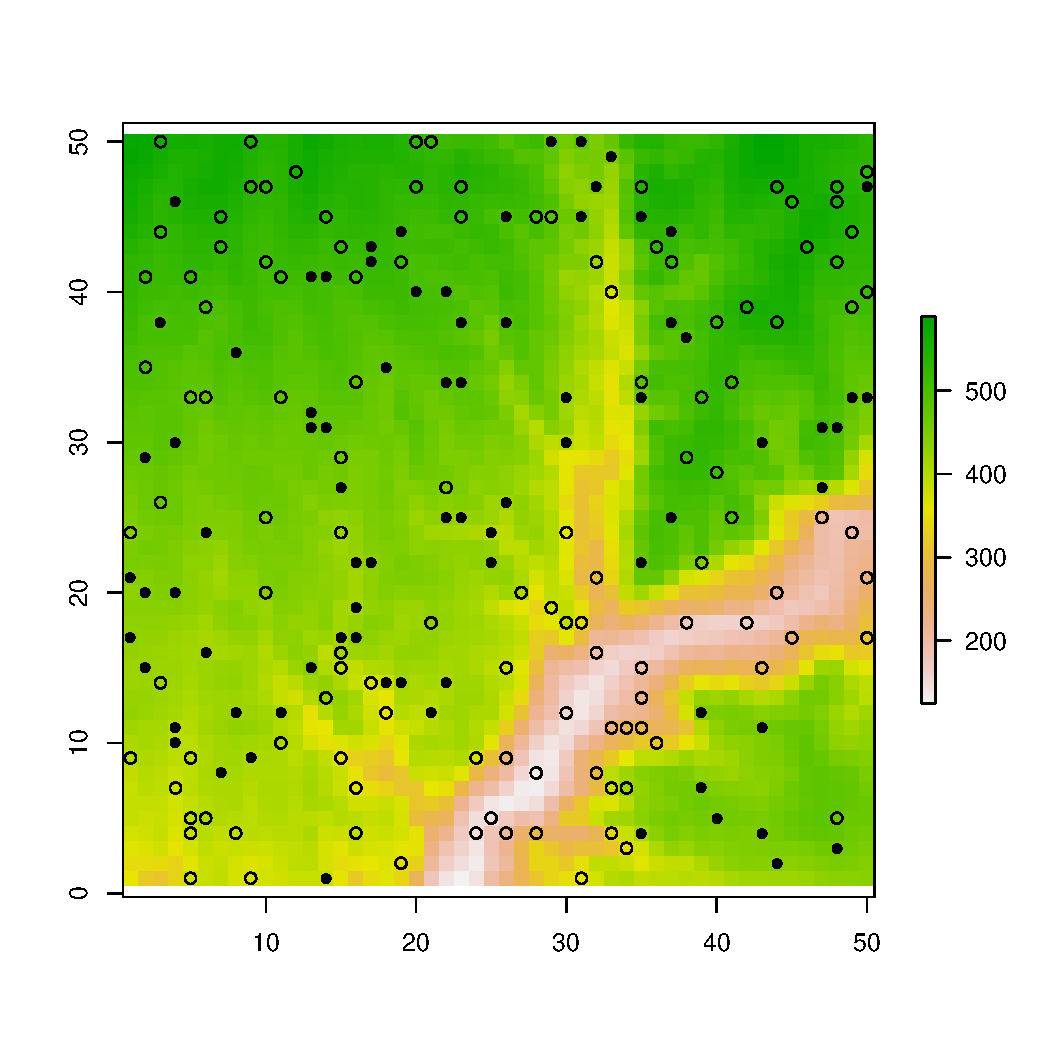
\includegraphics[width=8cm]{figures/observations-binomial.pdf}
  \caption{\textbf{Observation points}. Presences (full circles) and absences (empty
    circles) are localized on the altitude map (in m).}
  \label{fig:observations-binomial}
\end{figure}

\subsubsection{Parameter inference using the \texttt{hSDM.binomial()} function}

The \texttt{hSDM.binomial()} function performs a Binomial logistic regression in a
Bayesian framework. Before using this function we need to prepare a bit the data for
predictions. We want to have predictions on the whole landscape, not only at observation
points. To directly obtain these predictions, we can create a data frame including
altitudinal data on the whole landscape. This data frame will be used for the
\texttt{suitability.pred} argument. The data frame for predictions must include the same
column names as those used in the formula for the \texttt{suitability} argument
(i.e. ``alt'' and ``alt2'' in our example).

\begin{knitrout}\small
\definecolor{shadecolor}{rgb}{0.969, 0.969, 0.969}\color{fgcolor}\begin{kframe}
\begin{alltt}
\hlstd{data.pred} \hlkwb{<-} \hlkwd{data.frame}\hlstd{(}\hlkwc{alt}\hlstd{=}\hlkwd{values}\hlstd{(alt),}\hlkwc{alt2}\hlstd{=(}\hlkwd{values}\hlstd{(alt))}\hlopt{^}\hlnum{2}\hlstd{)}
\end{alltt}
\end{kframe}
\end{knitrout}


We can now call the \texttt{hSDM.binomial()} function. Setting parameter \texttt{save.p}
to 1, we can save in memory the MCMC values for predictions. These values can be used to compute
several statistics for each predictions (mean, median, 95\% quantiles). For example, mean
and 95\% quantiles are useful to estimate the uncertainty around the mean predictions.     

\begin{knitrout}\small
\definecolor{shadecolor}{rgb}{0.969, 0.969, 0.969}\color{fgcolor}\begin{kframe}
\begin{alltt}
\hlstd{mod.hSDM.binomial} \hlkwb{<-} \hlkwd{hSDM.binomial}\hlstd{(}\hlkwc{presences}\hlstd{=data.obs}\hlopt{$}\hlstd{Y,}
                                   \hlkwc{trials}\hlstd{=data.obs}\hlopt{$}\hlstd{trials,}
                                   \hlkwc{suitability}\hlstd{=}\hlopt{~}\hlstd{alt}\hlopt{+}\hlstd{alt2,}
                                   \hlkwc{data}\hlstd{=data.obs,}
                                   \hlkwc{suitability.pred}\hlstd{=data.pred,}
                                   \hlkwc{burnin}\hlstd{=}\hlnum{1000}\hlstd{,} \hlkwc{mcmc}\hlstd{=}\hlnum{1000}\hlstd{,} \hlkwc{thin}\hlstd{=}\hlnum{1}\hlstd{,}
                                   \hlkwc{beta.start}\hlstd{=}\hlnum{0}\hlstd{,}
                                   \hlkwc{mubeta}\hlstd{=}\hlnum{0}\hlstd{,} \hlkwc{Vbeta}\hlstd{=}\hlnum{1.0E6}\hlstd{,}
                                   \hlkwc{seed}\hlstd{=}\hlnum{1234}\hlstd{,} \hlkwc{verbose}\hlstd{=}\hlnum{1}\hlstd{,} \hlkwc{save.p}\hlstd{=}\hlnum{1}\hlstd{)}
\end{alltt}
\end{kframe}
\end{knitrout}


\subsubsection{Analysis of the results}

The \texttt{hSDM.binomial()} function returns an MCMC (Markov chain Monte Carlo) for each
parameter of the model and also for the model deviance. To obtain parameter estimates,
MCMC values can be summarized through a call to the \texttt{summary()} function from the
\textbf{coda} package. We can check that the values of the target parameters
$\beta_0=1$, $\beta_1=2$ and $\beta_2=-4$ are within the 95\% confidence interval of
the parameter estimates.

\begin{knitrout}\small
\definecolor{shadecolor}{rgb}{0.969, 0.969, 0.969}\color{fgcolor}\begin{kframe}
\begin{alltt}
\hlkwd{summary}\hlstd{(mod.hSDM.binomial}\hlopt{$}\hlstd{mcmc)}
\end{alltt}
\begin{verbatim}
## 
## Iterations = 1001:2000
## Thinning interval = 1 
## Number of chains = 1 
## Sample size per chain = 1000 
## 
## 1. Empirical mean and standard deviation for each variable,
##    plus standard error of the mean:
## 
##                    Mean    SD Naive SE Time-series SE
## beta.(Intercept)   1.18 0.231  0.00732         0.0215
## beta.alt           1.57 0.556  0.01758         0.0821
## beta.alt2         -3.89 0.694  0.02194         0.1116
## Deviance         196.27 2.430  0.07685         0.2225
## 
## 2. Quantiles for each variable:
## 
##                     2.5%    25%    50%    75%  97.5%
## beta.(Intercept)   0.735   1.02   1.16   1.34   1.62
## beta.alt           0.468   1.16   1.57   1.97   2.64
## beta.alt2         -5.200  -4.37  -3.88  -3.37  -2.41
## Deviance         193.428 194.50 195.67 197.53 202.85
\end{verbatim}
\end{kframe}
\end{knitrout}


Parameters estimates can be compared to results obtained with the \texttt{glm()} function.

\begin{knitrout}\small
\definecolor{shadecolor}{rgb}{0.969, 0.969, 0.969}\color{fgcolor}\begin{kframe}
\begin{alltt}
\hlcom{#== glm results for comparison}
\hlstd{mod.glm} \hlkwb{<-} \hlkwd{glm}\hlstd{(}\hlkwd{cbind}\hlstd{(Y,trials}\hlopt{-}\hlstd{Y)}\hlopt{~}\hlstd{alt}\hlopt{+}\hlstd{alt2,}\hlkwc{family}\hlstd{=}\hlstr{"binomial"}\hlstd{,}\hlkwc{data}\hlstd{=data.obs)}
\hlkwd{summary}\hlstd{(mod.glm)}
\end{alltt}
\begin{verbatim}
## 
## Call:
## glm(formula = cbind(Y, trials - Y) ~ alt + alt2, family = "binomial", 
##     data = data.obs)
## 
## Deviance Residuals: 
##    Min      1Q  Median      3Q     Max  
## -1.766  -0.797   0.000   0.799   3.112  
## 
## Coefficients:
##             Estimate Std. Error z value Pr(>|z|)    
## (Intercept)    1.186      0.241    4.92  8.6e-07 ***
## alt            1.475      0.538    2.74   0.0061 ** 
## alt2          -3.736      0.735   -5.08  3.7e-07 ***
## ---
## Signif. codes:  0 '***' 0.001 '**' 0.01 '*' 0.05 '.' 0.1 ' ' 1
## 
## (Dispersion parameter for binomial family taken to be 1)
## 
##     Null deviance: 276.54  on 199  degrees of freedom
## Residual deviance: 193.15  on 197  degrees of freedom
## AIC: 199.1
## 
## Number of Fisher Scoring iterations: 8
\end{verbatim}
\end{kframe}
\end{knitrout}


MCMC can also be graphically summarized with a call to the \texttt{plot.mcmc()} function,
also in the \textbf{coda} package. MCMC are plotted with a trace of the sampled output and
a density estimate for each variable in the chain (Fig.~\ref{fig:mcmc-binomial}). This
plot can be used to visually check that the chains have converged.

\begin{knitrout}\small
\definecolor{shadecolor}{rgb}{0.969, 0.969, 0.969}\color{fgcolor}\begin{kframe}
\begin{alltt}
\hlkwd{plot}\hlstd{(mod.hSDM.binomial}\hlopt{$}\hlstd{mcmc)}
\end{alltt}
\end{kframe}
\end{knitrout}


\begin{figure}[!h] 
  \centering 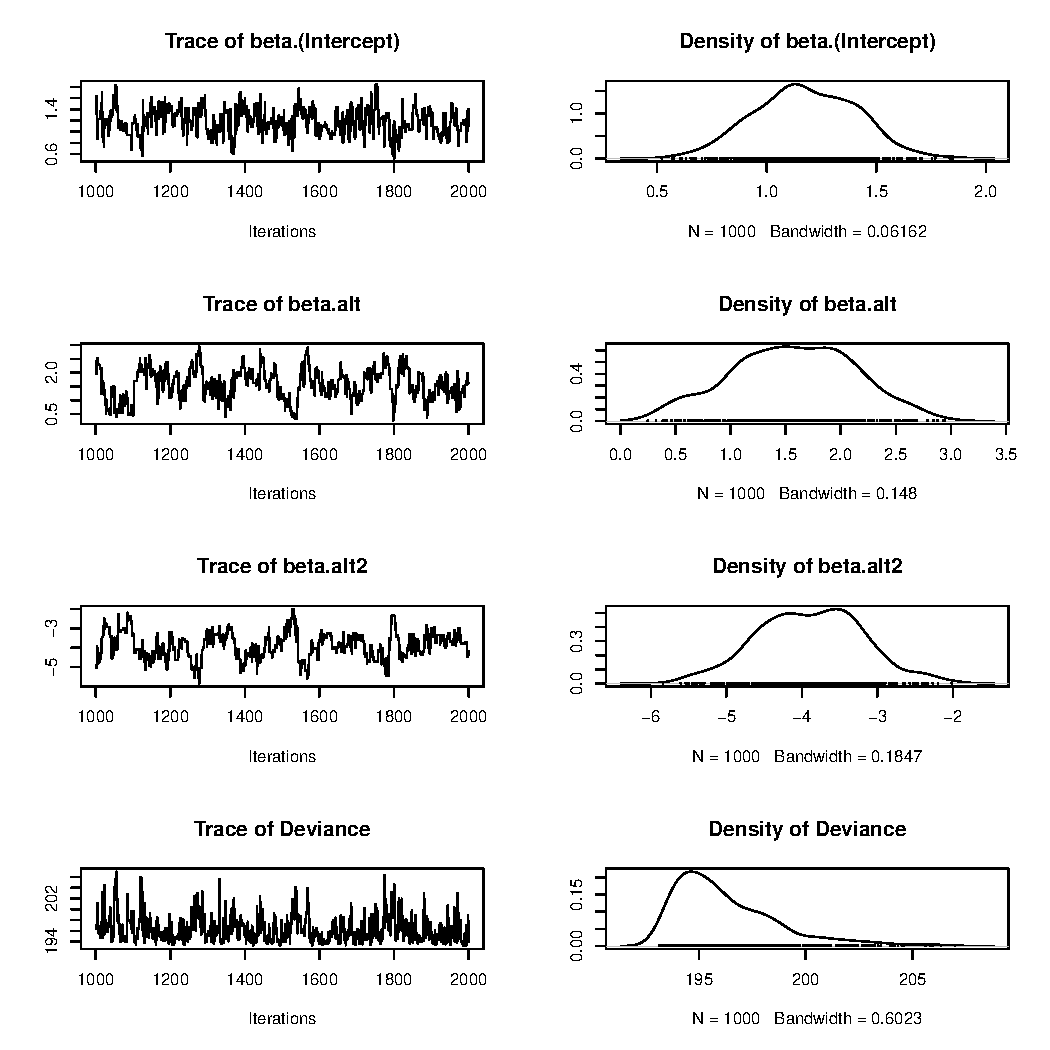
\includegraphics[width=\textwidth]{figures/mcmc-binomial.pdf}
  \caption{\textbf{Trace and density estimate for each variable of the MCMC}.}
  \label{fig:mcmc-binomial}
\end{figure}

The \texttt{hSDM.binomial()} function also returns two other objects. The first one,
\texttt{prob.p.latent}, is the predictive posterior mean of the latent variable
$\theta$ (the probability of presence) for each observation. 

\begin{knitrout}\small
\definecolor{shadecolor}{rgb}{0.969, 0.969, 0.969}\color{fgcolor}\begin{kframe}
\begin{alltt}
\hlkwd{str}\hlstd{(mod.hSDM.binomial}\hlopt{$}\hlstd{prob.p.latent)}
\end{alltt}
\begin{verbatim}
##  num [1:200] 0.17046 0.4498 0.6823 0.00542 0.05014 ...
\end{verbatim}
\begin{alltt}
\hlkwd{summary}\hlstd{(mod.hSDM.binomial}\hlopt{$}\hlstd{prob.p.latent)}
\end{alltt}
\begin{verbatim}
##    Min. 1st Qu.  Median    Mean 3rd Qu.    Max. 
##   0.000   0.184   0.572   0.465   0.731   0.789
\end{verbatim}
\end{kframe}
\end{knitrout}


The second one, \texttt{prob.p.pred} is the set of sampled values from the predictive
posterior (if parameter \texttt{save.p} is set to 1) or the predictive posterior mean (if
\texttt{save.p} is set to 0) for each prediction. In our example, \texttt{save.p} is set
to 1 and \texttt{prob.p.pred} is an \texttt{mcmc} object. Values in \texttt{prob.p.pred} can be
used to plot the predicted probability of presence on the whole landscape and the
uncertainty associated to the predictions (Fig~\ref{fig:predictions-binomial}).

\begin{knitrout}\small
\definecolor{shadecolor}{rgb}{0.969, 0.969, 0.969}\color{fgcolor}\begin{kframe}
\begin{alltt}
\hlcom{# Create a raster for predictions}
\hlstd{theta.pred.mean} \hlkwb{<-} \hlkwd{raster}\hlstd{(theta)}
\hlcom{# Create rasters for uncertainty}
\hlstd{theta.pred.2.5} \hlkwb{<-} \hlstd{theta.pred.97.5} \hlkwb{<-} \hlkwd{raster}\hlstd{(theta)}
\hlcom{# Attribute predicted values to raster cells}
\hlstd{theta.pred.mean[]} \hlkwb{<-} \hlkwd{apply}\hlstd{(mod.hSDM.binomial}\hlopt{$}\hlstd{prob.p.pred,}\hlnum{2}\hlstd{,mean)}
\hlstd{theta.pred.2.5[]} \hlkwb{<-} \hlkwd{apply}\hlstd{(mod.hSDM.binomial}\hlopt{$}\hlstd{prob.p.pred,}\hlnum{2}\hlstd{,quantile,}\hlnum{0.025}\hlstd{)}
\hlstd{theta.pred.97.5[]} \hlkwb{<-} \hlkwd{apply}\hlstd{(mod.hSDM.binomial}\hlopt{$}\hlstd{prob.p.pred,}\hlnum{2}\hlstd{,quantile,}\hlnum{0.975}\hlstd{)}
\hlcom{# Plot the predicted probability of presence and uncertainty}
\hlkwd{plot}\hlstd{(theta.pred.mean,}\hlkwc{col}\hlstd{=}\hlkwd{rev}\hlstd{(}\hlkwd{heat.colors}\hlstd{(}\hlnum{255}\hlstd{)))}
\hlkwd{plot}\hlstd{(theta.pred.2.5,}\hlkwc{col}\hlstd{=}\hlkwd{rev}\hlstd{(}\hlkwd{heat.colors}\hlstd{(}\hlnum{255}\hlstd{)))}
\hlkwd{plot}\hlstd{(theta.pred.97.5,}\hlkwc{col}\hlstd{=}\hlkwd{rev}\hlstd{(}\hlkwd{heat.colors}\hlstd{(}\hlnum{255}\hlstd{)))}
\end{alltt}
\end{kframe}
\end{knitrout}


\begin{figure}[!h] 
  \centering 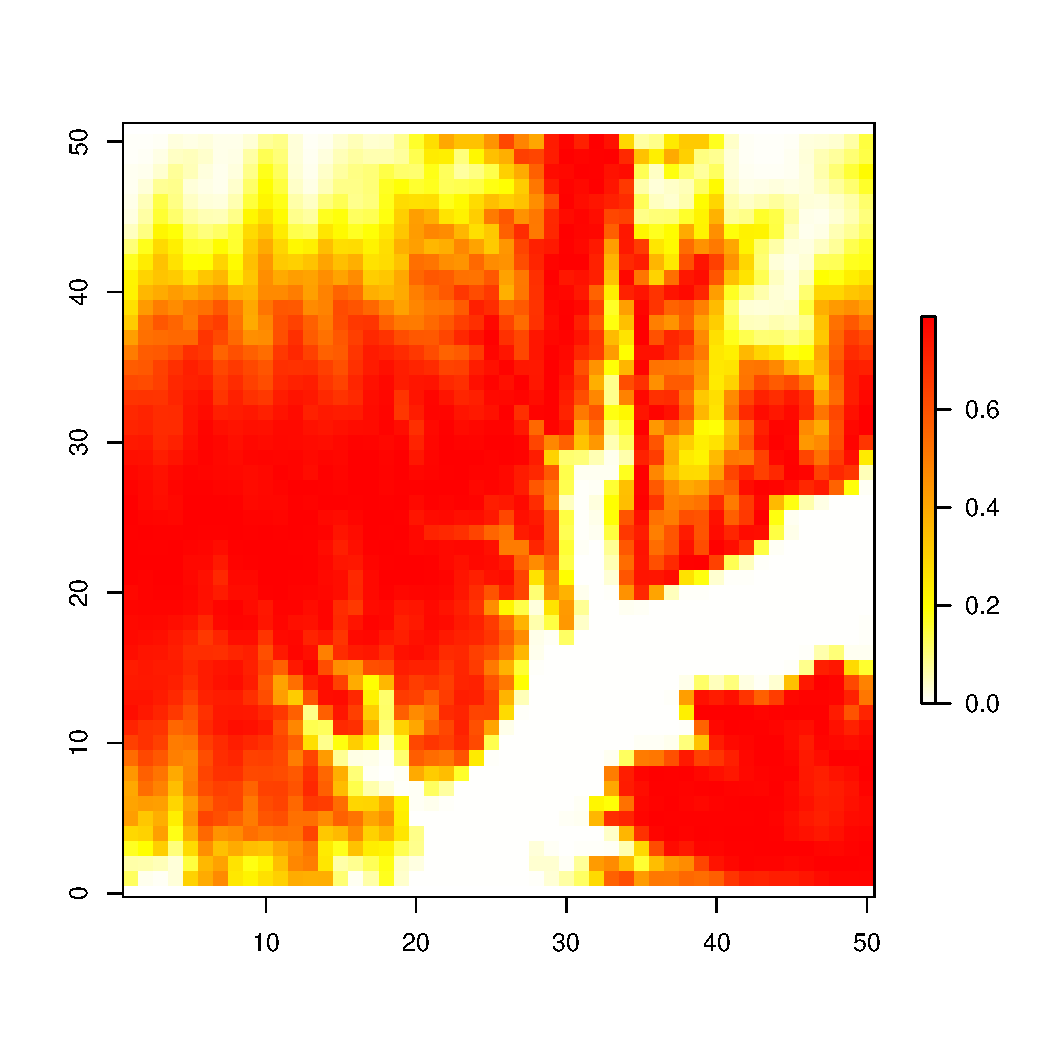
\includegraphics[width=8cm]{figures/predictions-binomial1.pdf} \\
  \begin{tabular}{cc}
    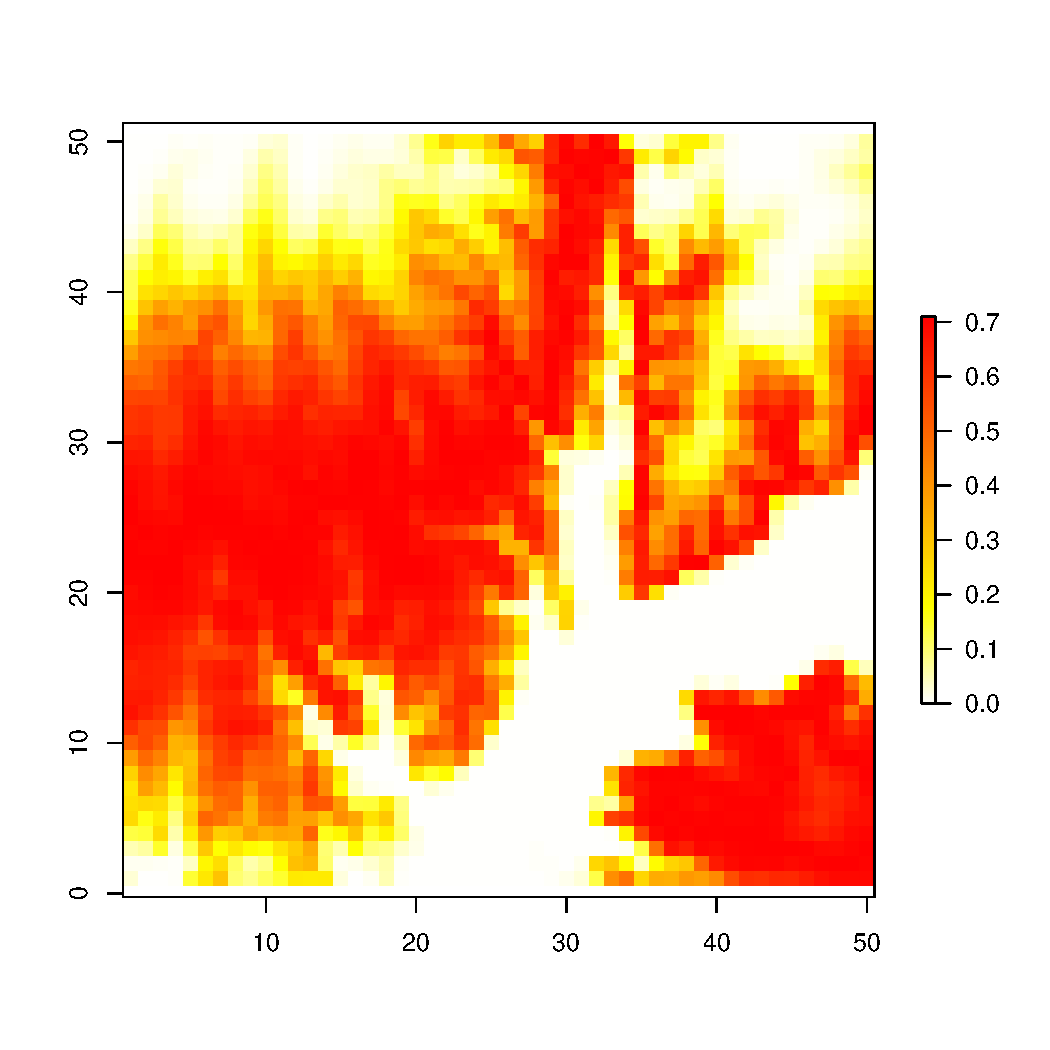
\includegraphics[width=8cm]{figures/predictions-binomial2.pdf} &
    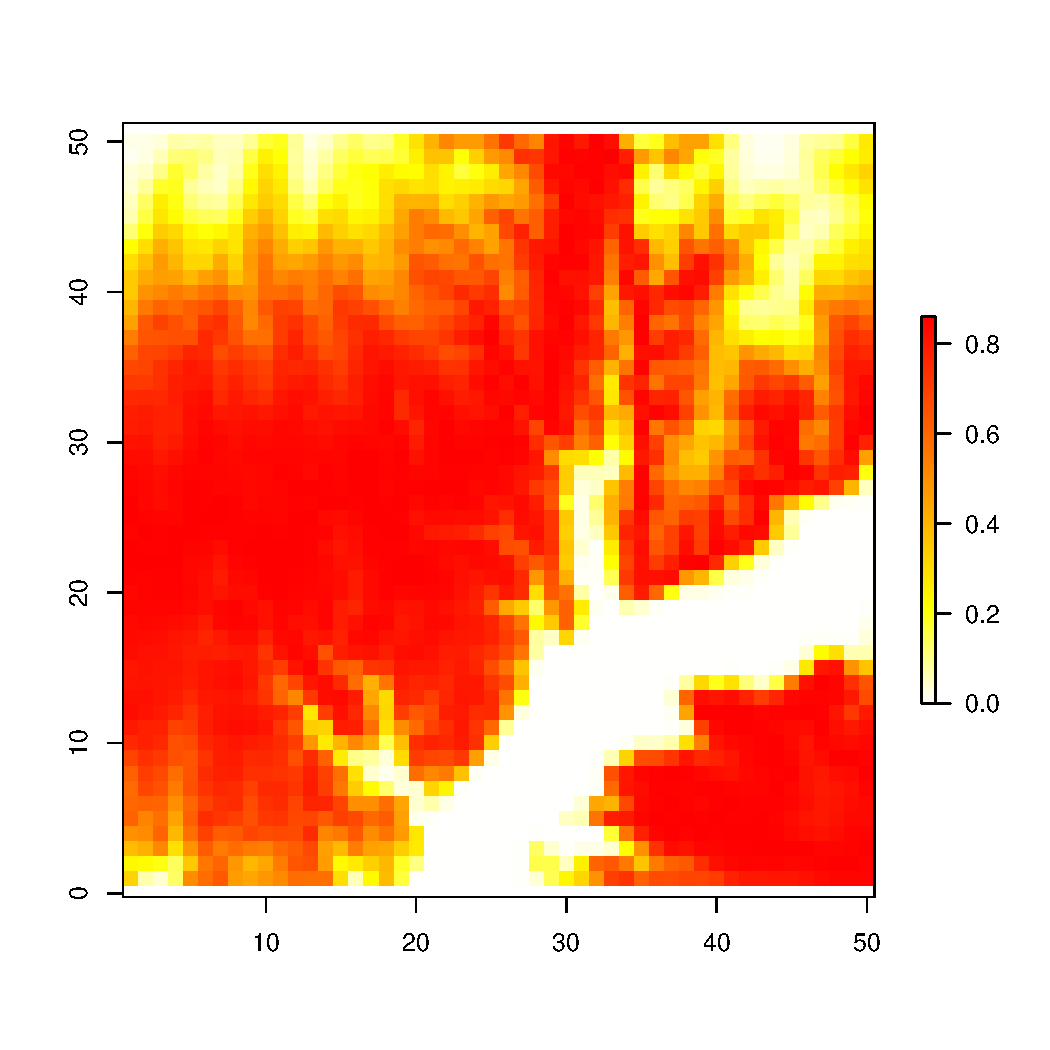
\includegraphics[width=8cm]{figures/predictions-binomial3.pdf} \\
  \end{tabular}
  
  \caption{\textbf{Predicted probability of presence and uncertainty of predictions}. Mean
    probability of presence (top), predictions at 2.5\% quantile (bottom left) and 97.5\%
    quantile (bottom right) can be plotted from the \texttt{mcmc} object
    \texttt{plot.p.pred} returned by function \texttt{hSDM.binomial()}.}
  
  \label{fig:predictions-binomial}
  
\end{figure}

In our example, we can compare the predictions to the initial probability of presence
computed from our model to check that our predictions are correct
(Fig.~\ref{fig:pred-obs-binomial}).

\begin{knitrout}\small
\definecolor{shadecolor}{rgb}{0.969, 0.969, 0.969}\color{fgcolor}\begin{kframe}
\begin{alltt}
\hlcom{# Comparing predictions to initial values}
\hlkwd{plot}\hlstd{(theta[],theta.pred.mean[],}\hlkwc{cex.lab}\hlstd{=}\hlnum{1.4}\hlstd{)}
\hlkwd{abline}\hlstd{(}\hlkwc{a}\hlstd{=}\hlnum{0}\hlstd{,}\hlkwc{b}\hlstd{=}\hlnum{1}\hlstd{,}\hlkwc{col}\hlstd{=}\hlstr{"red"}\hlstd{,}\hlkwc{lwd}\hlstd{=}\hlnum{2}\hlstd{)}
\end{alltt}
\end{kframe}
\end{knitrout}


\begin{figure}[!h] 
  \centering 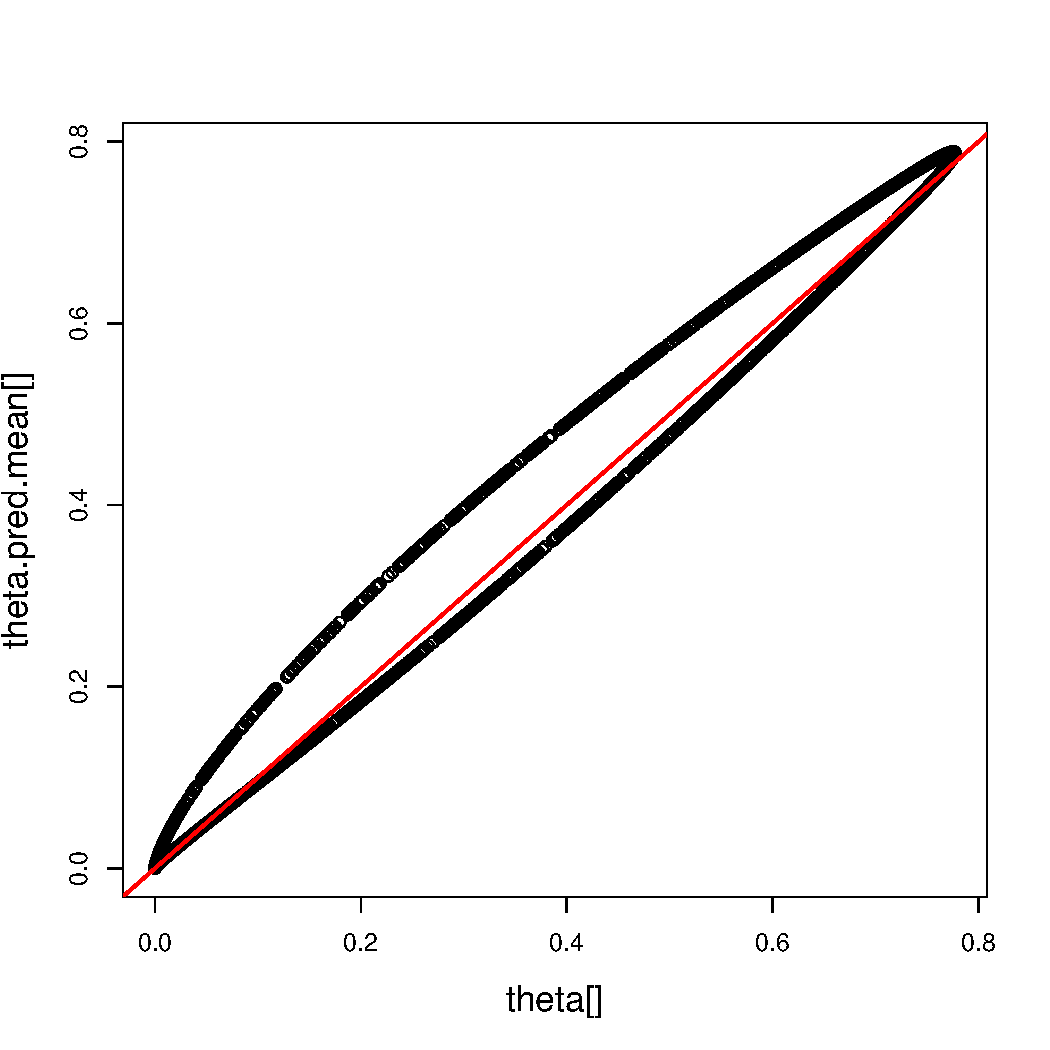
\includegraphics[width=8cm]{figures/pred-obs-binomial.pdf}
  
  \caption{\textbf{Predicted vs. initial probabilities of presence}. Initial probabilities
    of presence are computed from the Binomial logistic regression model with fixed
    parameters.}
  
  \label{fig:pred-obs-binomial}
  
\end{figure}

\subsection{Site-occupancy model}

\subsubsection{Mathematical formulation}

Occurrence of a species is typically not observed perfectly. Species traits,
survey-specific conditions and site-specific characteristics may influence species
detection probability which is often $<1$ \citep{Chen2013}. Thus, observations might
include false absences. For example, the habitat can be suitable and the species present
but individuals have not been seen during the census. Or the habitat can be suitable but
the species has not dispersed yet to the site (typical example for plant species, see
\citet{Latimer2006}) or was not present on the site at the moment of the observation
(typical example for animal species such as birds, see \citet{Kery2005}). Treating
observed occurrence and species distributions as the true occurrence and distribution,
failing to make amendments for imperfect detection, may lead to problems in species
distribution studies, habitat models and biodiversity management
\citep{Latimer2006,Lahoz-Monfort2014,Kery2008}.

New classes of models, called site-occupancy models, were developed to solve the problems
created by imperfect detection \citep{MacKenzie2002}. These models combine two processes,
an ecological process which describes habitat suitability and an observation process which
takes into account imperfect detection. Site-occupancy models use information from
repeated observations at each site to estimate detectability. Detectability may vary with
site characteristics (e.g., habitat variables) or survey characteristics (e.g., weather
conditions), whereas occupancy relates only to site characteristics.

Let's consider the random variable $z_{i(jt)}$ (abbreviated $z_i$) describing habitat
suitability for observation $i$ at site $j$ and at time $t$. The random variable $z_i$ can
take value 1 or 0 depending on the fact that the habitat at site $j$ and at time $t$ is
suitable ($z_i=1$) or not ($z_i=0$). Habitat at site $j$ and time $t$ is described by
environmental variables $X_{i(jt)}$. Random variable $z_i$ can be assumed to follow a
Bernoulli distribution of parameter $\theta_i$ (Eq.~\ref{eq:siteocc}). In this case,
$\theta_i$ is the probability that the habitat is suitable. Let's consider also the random
variable $y_{i(jt)}$ (abbreviated $y_i$) representing the total number of presences of a
species after several visits $v_{i(jt)}$ (abbreviated $v_i$) at a particular site $j$ at
time $t$. Again, $t$ can indicate a day, a year, etc. thus allowing several visits at time
$t$. The species is observed ($y_i \geq 1$) only if the habitat is suitable ($z=1$). The
species is unobserved ($y_i=0$) if the habitat is not suitable ($z_i=0$) or if the habitat
is suitable ($z_i=1$) but the detection probability $\delta_{i(jt)}$ (abbreviated
$\delta_i$) is inferior to 1. Thus, the total number of presences $y_i$ is assumed to
follow a Binomial distribution with parameters $z_i \delta_i$ and $v_i$. Using a logit
link function, $\delta_i$ can be expressed as a linear model combining explicative
variables $W_{i(jt)}$ and parameters $\gamma$ (Eq.~\ref{eq:siteocc}). Typically,
explicative variables $W_{i(jt)}$ are site characteristics (e.g., habitat variables) or
survey characteristics (e.g., weather conditions). The function \texttt{hSDM.siteocc()}
estimates the parameters $\beta$ and $\gamma$ of such a model.

\begin{equation}
  \begin{tabular}{c}
    \textbf{Ecological process:}\\
    $z_i \sim \mathcal{B}ernoulli(\theta_i)$ \\
    $\logit(\theta_i) = X_{i(jt)} \beta$\\
    ~ \\
    \textbf{Observation process:}\\
    $y_i \sim \mathcal{B}inomial(z_i \delta_i, v_i)$ \\
    $\logit(\delta_i) = W_{i(jt)} \gamma$ \\
  \end{tabular}
  \label{eq:siteocc}
\end{equation}

\subsubsection{Data generation}

To explore the characteristics of the \texttt{hSDM.siteocc()} function, we can generate a
new virtual data-set on the basis of the site-occupancy model described above
(Eq.~\ref{eq:siteocc}). In most general cases, protocol experiments would include severals
visits with varying survey conditions (e.g. weather conditions) to several sites with
fixed sites characteristics (e.g. habitat variables). We will generate virtual data
following this protocole and using the altitudinal data used in the previous example for
the Binomial model (Sec.~\ref{sec:binomial}).

We draw at random the number of visits at each observation point used in the previous
example (see Fig.~\ref{fig:observations-binomial} of Sec.~\ref{sec:binomial}).

\begin{knitrout}\small
\definecolor{shadecolor}{rgb}{0.969, 0.969, 0.969}\color{fgcolor}\begin{kframe}
\begin{alltt}
\hlcom{# Number of visits associated to each observation point}
\hlkwd{set.seed}\hlstd{(seed)}
\hlstd{v} \hlkwb{<-} \hlkwd{rpois}\hlstd{(nobspt,}\hlnum{2}\hlstd{)}
\hlstd{v[v}\hlopt{==}\hlnum{0}\hlstd{]} \hlkwb{<-} \hlnum{1}
\hlcom{# Vector of observation points}
\hlstd{obspt} \hlkwb{<-} \hlkwd{vector}\hlstd{()}
\hlkwa{for} \hlstd{(i} \hlkwa{in} \hlnum{1}\hlopt{:}\hlstd{nobspt) \{}
    \hlstd{obspt} \hlkwb{<-} \hlkwd{c}\hlstd{(obspt,}\hlkwd{rep}\hlstd{(i,v[i]))}
\hlstd{\}}
\end{alltt}
\end{kframe}
\end{knitrout}


We fix the survey conditions for each visit depending on two explicative variables $w_1$
and $w_2$ which will explain the observability of the species. We also fix the intercept
and the effects of these two variables: $\gamma_0=0.2$, $\gamma_1=0.5$ and $\gamma_2=0.5$
for determining the detection probability.

\begin{knitrout}\small
\definecolor{shadecolor}{rgb}{0.969, 0.969, 0.969}\color{fgcolor}\begin{kframe}
\begin{alltt}
\hlcom{# Explicative variables for observation process}
\hlstd{nobs} \hlkwb{<-} \hlkwd{sum}\hlstd{(v)}
\hlkwd{set.seed}\hlstd{(seed)}
\hlstd{w1} \hlkwb{<-} \hlkwd{rnorm}\hlstd{(}\hlkwc{n}\hlstd{=nobs,}\hlnum{0}\hlstd{,}\hlnum{1}\hlstd{)}
\hlkwd{set.seed}\hlstd{(}\hlnum{2}\hlopt{*}\hlstd{seed)}
\hlstd{w2} \hlkwb{<-} \hlkwd{rnorm}\hlstd{(}\hlkwc{n}\hlstd{=nobs,}\hlnum{0}\hlstd{,}\hlnum{1}\hlstd{)}
\hlstd{W} \hlkwb{<-} \hlkwd{cbind}\hlstd{(}\hlkwd{rep}\hlstd{(}\hlnum{1}\hlstd{,nobs),w1,w2)}
\hlcom{# Target parameters for observation process}
\hlstd{gamma.target} \hlkwb{<-} \hlkwd{matrix}\hlstd{(}\hlkwd{c}\hlstd{(}\hlnum{0.2}\hlstd{,}\hlnum{0.5}\hlstd{,}\hlnum{0.5}\hlstd{),}\hlkwc{ncol}\hlstd{=}\hlnum{1}\hlstd{)}
\end{alltt}
\end{kframe}
\end{knitrout}


Using covariates and parameters for the two processes, we compute the probability that
the habitat is suitable ($\theta_i$) and the species detection probability
($\delta_i$). We also draw the random variables $z_i$ and $y_i$ and construct the
observation data-set.

\begin{knitrout}\small
\definecolor{shadecolor}{rgb}{0.969, 0.969, 0.969}\color{fgcolor}\begin{kframe}
\begin{alltt}
\hlcom{# Ecological process (suitability)}
\hlstd{logit.theta.obspt} \hlkwb{<-} \hlstd{X} \hlopt \hlstd{beta.target}
\hlstd{theta.obspt} \hlkwb{<-} \hlkwd{inv.logit}\hlstd{(logit.theta.obspt)}
\hlkwd{set.seed}\hlstd{(seed)}
\hlstd{Z} \hlkwb{<-} \hlkwd{rbinom}\hlstd{(nobspt,}\hlnum{1}\hlstd{,theta.obspt)}

\hlcom{# Observation process (detectability)}
\hlstd{logit.delta.obs} \hlkwb{<-} \hlstd{W} \hlopt \hlstd{gamma.target}
\hlstd{delta.obs} \hlkwb{<-} \hlkwd{inv.logit}\hlstd{(logit.delta.obs)}
\hlkwd{set.seed}\hlstd{(seed)}
\hlcom{# Y <- rbinom(nobs,1,delta.obs*Z[obspt])}
\hlstd{Y} \hlkwb{<-} \hlkwd{rbinom}\hlstd{(nobs,}\hlnum{1}\hlstd{,}\hlnum{0.8}\hlopt{*}\hlstd{Z[obspt])}

\hlcom{# Spatial entity (raster cells) associated to each observation}
\hlstd{cell.obspt} \hlkwb{<-} \hlkwd{extract}\hlstd{(alt,obs,}\hlkwc{cellnumbers}\hlstd{=}\hlnum{TRUE}\hlstd{)[,}\hlstr{"cells"}\hlstd{]}
\hlstd{cell.obs} \hlkwb{<-} \hlstd{cell.obspt[obspt]}
\hlcom{# cell.obs <- as.numeric(as.factor(cell.obs)) # from 1 to ncell, not necessary}

\hlcom{# Data-sets}
\hlstd{data.obs} \hlkwb{<-} \hlkwd{data.frame}\hlstd{(Y,w1,w2,}\hlkwc{cell}\hlstd{=cell.obs)}
\hlstd{data.suit} \hlkwb{<-} \hlkwd{data.frame}\hlstd{(}\hlkwc{alt}\hlstd{=X[,}\hlnum{2}\hlstd{],}\hlkwc{alt2}\hlstd{=X[,}\hlnum{3}\hlstd{])}
\end{alltt}
\end{kframe}
\end{knitrout}

\subsubsection{Parameter inference using the \texttt{hSDM.siteocc()} function}

The \texttt{hSDM.siteocc()} function estimates the parameter of a site-occupancy model in
a Bayesian framework.

\begin{knitrout}\small
\definecolor{shadecolor}{rgb}{0.969, 0.969, 0.969}\color{fgcolor}\begin{kframe}
\begin{alltt}
\hlstd{mod.hSDM.siteocc} \hlkwb{<-} \hlkwd{hSDM.siteocc}\hlstd{(}\hlcom{# Observations}
                                 \hlkwc{presences}\hlstd{=data.obs}\hlopt{$}\hlstd{Y,}
                                 \hlcom{#observability=~w1+w2,}
                                 \hlkwc{observability}\hlstd{=}\hlopt{~}\hlnum{1}\hlstd{,}
                                 \hlkwc{spatial.entity}\hlstd{=data.obs}\hlopt{$}\hlstd{cell,}
                                 \hlkwc{data.observability}\hlstd{=data.obs,}
                                 \hlcom{# Habitat                                 }
                                 \hlkwc{suitability}\hlstd{=}\hlopt{~}\hlstd{alt}\hlopt{+}\hlstd{alt2,}
                                 \hlkwc{data.suitability}\hlstd{=data.suit,}
                                 \hlcom{# Predictions}
                                 \hlkwc{suitability.pred}\hlstd{=data.pred,}
                                 \hlcom{# Chains}
                                 \hlkwc{burnin}\hlstd{=}\hlnum{1000}\hlstd{,} \hlkwc{mcmc}\hlstd{=}\hlnum{1000}\hlstd{,} \hlkwc{thin}\hlstd{=}\hlnum{1}\hlstd{,}
                                 \hlcom{# Starting values}
                                 \hlkwc{beta.start}\hlstd{=}\hlnum{0}\hlstd{,}
                                 \hlkwc{gamma.start}\hlstd{=}\hlnum{0}\hlstd{,}
                                 \hlcom{# Priors}
                                 \hlkwc{mubeta}\hlstd{=}\hlnum{0}\hlstd{,} \hlkwc{Vbeta}\hlstd{=}\hlnum{1.0E6}\hlstd{,}
                                 \hlkwc{mugamma}\hlstd{=}\hlnum{0}\hlstd{,} \hlkwc{Vgamma}\hlstd{=}\hlnum{1.0E6}\hlstd{,}
                                 \hlcom{# Various}
                                 \hlkwc{seed}\hlstd{=}\hlnum{1234}\hlstd{,} \hlkwc{verbose}\hlstd{=}\hlnum{1}\hlstd{,} \hlkwc{save.p}\hlstd{=}\hlnum{0}\hlstd{)}
\end{alltt}
\end{kframe}
\end{knitrout}


\subsubsection{Analysis of the results}

\begin{knitrout}\small
\definecolor{shadecolor}{rgb}{0.969, 0.969, 0.969}\color{fgcolor}\begin{kframe}
\begin{alltt}
\hlkwd{summary}\hlstd{(mod.hSDM.siteocc}\hlopt{$}\hlstd{mcmc)}
\end{alltt}
\begin{verbatim}
## 
## Iterations = 1001:2000
## Thinning interval = 1 
## Number of chains = 1 
## Sample size per chain = 1000 
## 
## 1. Empirical mean and standard deviation for each variable,
##    plus standard error of the mean:
## 
##                      Mean    SD Naive SE Time-series SE
## beta.(Intercept)   -0.219 0.195  0.00617         0.0200
## beta.alt            0.151 0.182  0.00575         0.0166
## beta.alt2          -0.122 0.120  0.00378         0.0156
## gamma.(Intercept)   1.918 0.285  0.00901         0.0185
## Deviance          364.457 2.656  0.08399         0.2087
## 
## 2. Quantiles for each variable:
## 
##                      2.5%     25%     50%      75%    97.5%
## beta.(Intercept)   -0.562  -0.361  -0.213  -0.0661   0.1284
## beta.alt           -0.236   0.023   0.153   0.2689   0.4740
## beta.alt2          -0.410  -0.196  -0.111  -0.0249   0.0621
## gamma.(Intercept)   1.348   1.735   1.937   2.1174   2.4523
## Deviance          360.818 362.343 364.009 365.8364 371.0877
\end{verbatim}
\end{kframe}
\end{knitrout}


\begin{knitrout}\small
\definecolor{shadecolor}{rgb}{0.969, 0.969, 0.969}\color{fgcolor}\begin{kframe}
\begin{alltt}
\hlkwd{plot}\hlstd{(mod.hSDM.siteocc}\hlopt{$}\hlstd{mcmc)}
\end{alltt}
\end{kframe}
\end{knitrout}


\begin{figure}[!h] 
  \begin{center}
    \begin{tabular}{cc}
      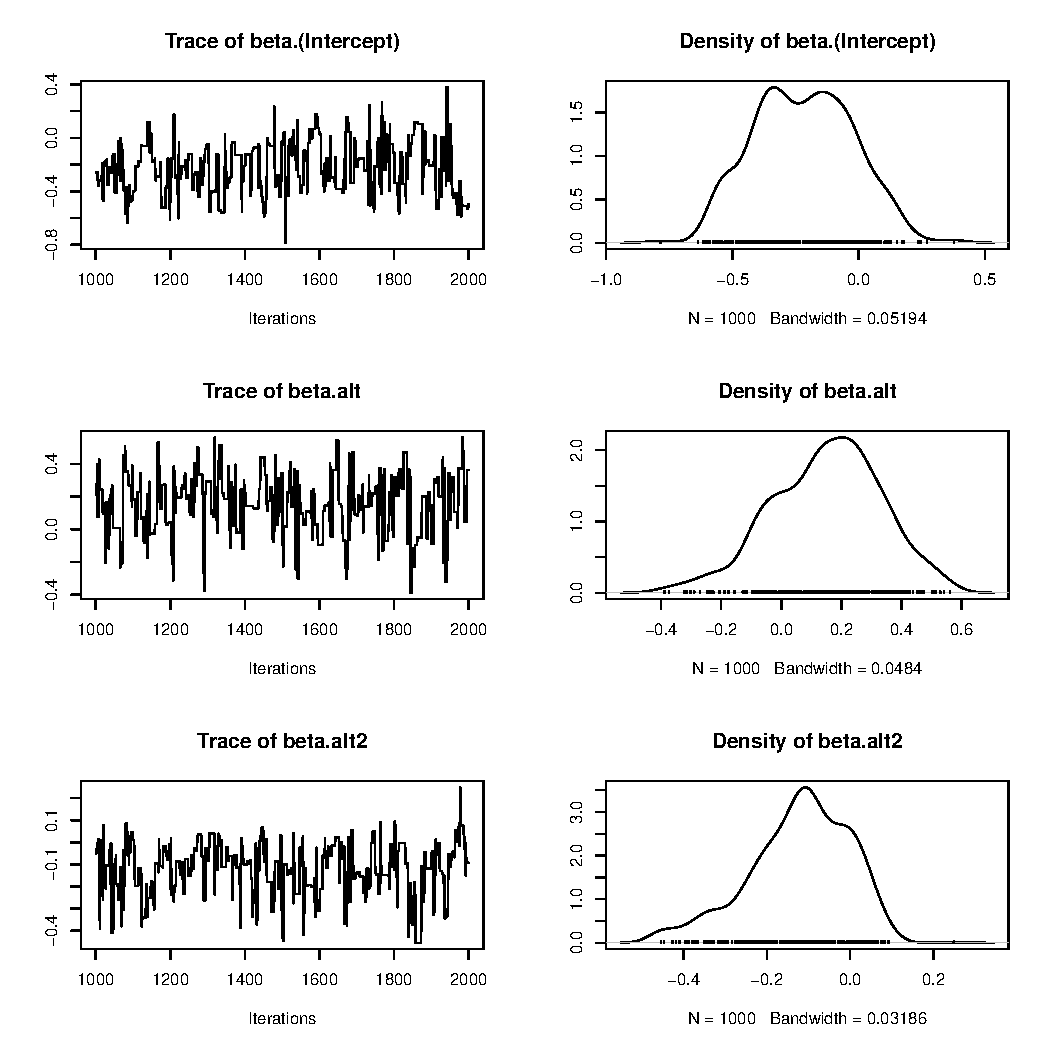
\includegraphics[width=8cm]{figures/mcmc-siteocc1.pdf} &
      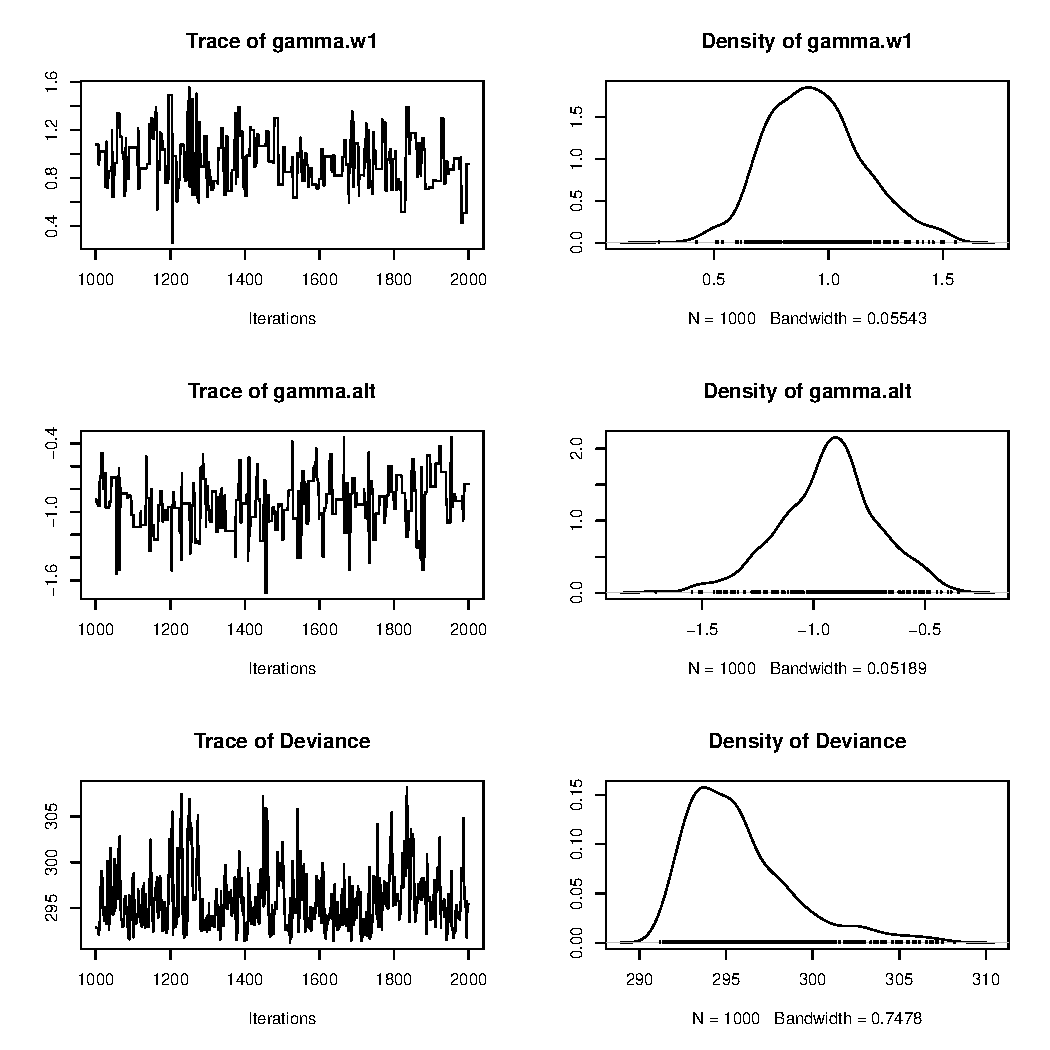
\includegraphics[width=8cm]{figures/mcmc-siteocc2.pdf} \\
    \end{tabular}
  \end{center}
  \caption{\textbf{Trace and density estimate for each variable of the MCMC}.}
  \label{fig:mcmc-siteocc}
\end{figure}

\begin{knitrout}\small
\definecolor{shadecolor}{rgb}{0.969, 0.969, 0.969}\color{fgcolor}\begin{kframe}
\begin{alltt}
\hlcom{# Create a raster for predictions}
\hlstd{theta.pred.mean} \hlkwb{<-} \hlkwd{raster}\hlstd{(theta)}
\hlcom{# Attribute predicted values to raster cells}
\hlstd{theta.pred.mean[]} \hlkwb{<-} \hlstd{mod.hSDM.siteocc}\hlopt{$}\hlstd{theta.pred}
\hlcom{# Plot the predicted probability of presence}
\hlkwd{plot}\hlstd{(theta.pred.mean,}\hlkwc{col}\hlstd{=}\hlkwd{rev}\hlstd{(}\hlkwd{heat.colors}\hlstd{(}\hlnum{255}\hlstd{)))}
\end{alltt}
\end{kframe}
\end{knitrout}


\begin{knitrout}\small
\definecolor{shadecolor}{rgb}{0.969, 0.969, 0.969}\color{fgcolor}\begin{kframe}
\begin{alltt}
\hlcom{# Comparing predictions to initial values}
\hlkwd{plot}\hlstd{(theta[],theta.pred.mean[],}\hlkwc{cex.lab}\hlstd{=}\hlnum{1.4}\hlstd{)}
\hlkwd{abline}\hlstd{(}\hlkwc{a}\hlstd{=}\hlnum{0}\hlstd{,}\hlkwc{b}\hlstd{=}\hlnum{1}\hlstd{,}\hlkwc{col}\hlstd{=}\hlstr{"red"}\hlstd{,}\hlkwc{lwd}\hlstd{=}\hlnum{2}\hlstd{)}
\end{alltt}
\end{kframe}
\end{knitrout}



\begin{figure}[!h] 
  \begin{tabular}{cc}
    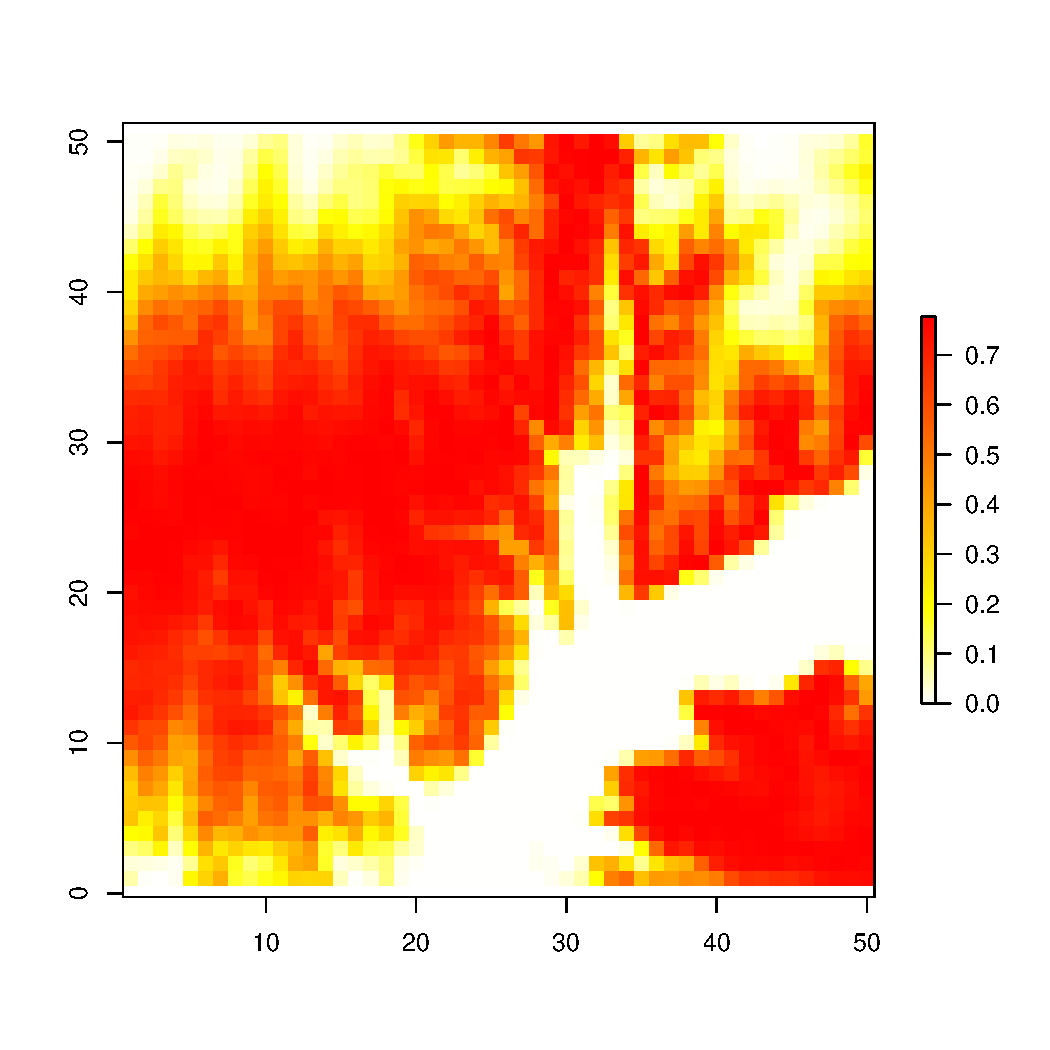
\includegraphics[width=8cm]{figures/theta-binomial.pdf} &
    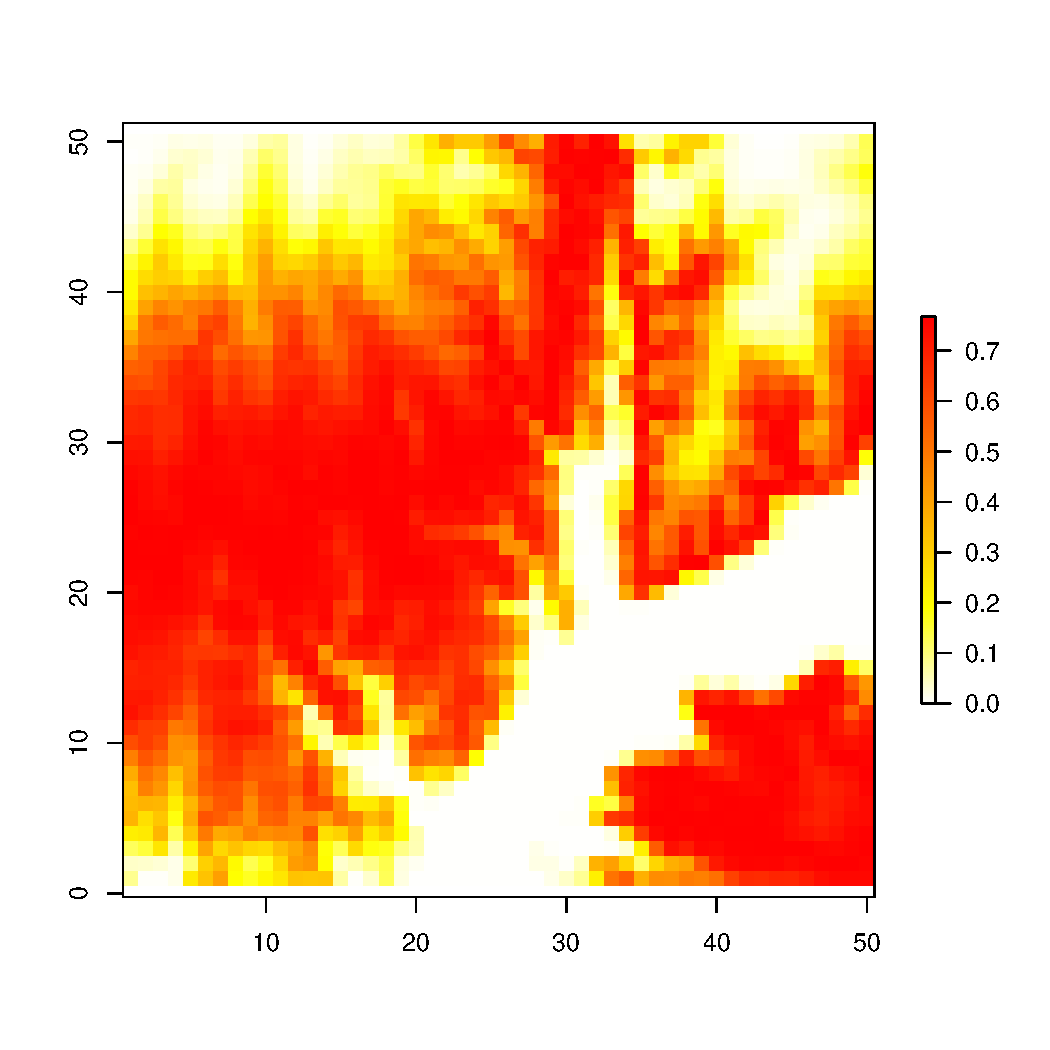
\includegraphics[width=8cm]{figures/predictions-siteocc.pdf} \\
  \end{tabular}
  \centering 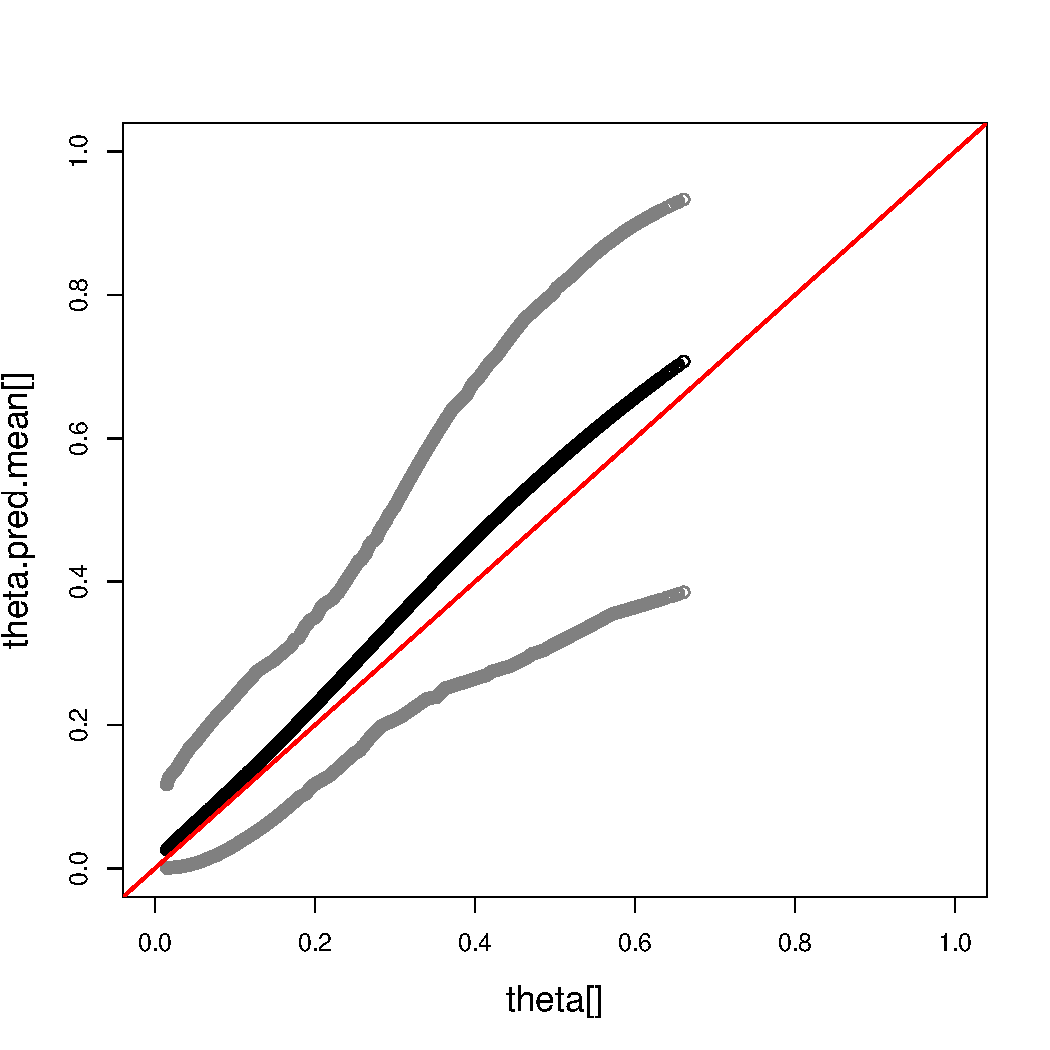
\includegraphics[width=8cm]{figures/pred-obs-siteocc.pdf} \\
  
  \caption{\textbf{Comparing predicted probability of presence with initial probabilities}}
  
  \label{fig:predictions-siteocc}
  
\end{figure}

Parameters estimates can be compared to results obtained with the \texttt{glm()} function
assuming a perfect detection.

\begin{knitrout}\small
\definecolor{shadecolor}{rgb}{0.969, 0.969, 0.969}\color{fgcolor}\begin{kframe}
\begin{alltt}
\hlcom{#== glm results for comparison}
\hlstd{data.obs.glm} \hlkwb{<-} \hlkwd{data.frame}\hlstd{(Y,}\hlkwc{alt}\hlstd{=X[obspt,}\hlnum{2}\hlstd{],}\hlkwc{alt2}\hlstd{=X[obspt,}\hlnum{3}\hlstd{])}
\hlstd{mod.glm} \hlkwb{<-} \hlkwd{glm}\hlstd{(Y}\hlopt{~}\hlstd{alt}\hlopt{+}\hlstd{alt2,}\hlkwc{family}\hlstd{=}\hlstr{"binomial"}\hlstd{,}\hlkwc{data}\hlstd{=data.obs.glm)}
\hlkwd{summary}\hlstd{(mod.glm)}
\end{alltt}
\begin{verbatim}
## 
## Call:
## glm(formula = Y ~ alt + alt2, family = "binomial", data = data.obs.glm)
## 
## Deviance Residuals: 
##    Min      1Q  Median      3Q     Max  
## -1.146  -1.046  -0.579   1.234   1.818  
## 
## Coefficients:
##             Estimate Std. Error z value Pr(>|z|)    
## (Intercept)  -0.0760     0.1372   -0.55     0.58    
## alt           0.0544     0.1943    0.28     0.78    
## alt2         -1.0477     0.2186   -4.79  1.6e-06 ***
## ---
## Signif. codes:  0 '***' 0.001 '**' 0.01 '*' 0.05 '.' 0.1 ' ' 1
## 
## (Dispersion parameter for binomial family taken to be 1)
## 
##     Null deviance: 534.91  on 416  degrees of freedom
## Residual deviance: 480.33  on 414  degrees of freedom
## AIC: 486.3
## 
## Number of Fisher Scoring iterations: 6
\end{verbatim}
\end{kframe}
\end{knitrout}


\begin{knitrout}\small
\definecolor{shadecolor}{rgb}{0.969, 0.969, 0.969}\color{fgcolor}\begin{kframe}
\begin{alltt}
\hlcom{# Create a raster for predictions}
\hlstd{theta.pred.glm} \hlkwb{<-} \hlkwd{raster}\hlstd{(theta)}
\hlcom{# Attribute predicted values to raster cells}
\hlstd{theta.pred.glm[]} \hlkwb{<-} \hlkwd{predict.glm}\hlstd{(mod.glm,}\hlkwc{newdata}\hlstd{=data.pred,}\hlkwc{type}\hlstd{=}\hlstr{"response"}\hlstd{)}
\hlcom{# Plot the predicted probability of presence}
\hlkwd{plot}\hlstd{(theta.pred.glm,}\hlkwc{col}\hlstd{=}\hlkwd{rev}\hlstd{(}\hlkwd{heat.colors}\hlstd{(}\hlnum{255}\hlstd{)))}
\end{alltt}
\end{kframe}
\end{knitrout}


\begin{knitrout}\small
\definecolor{shadecolor}{rgb}{0.969, 0.969, 0.969}\color{fgcolor}\begin{kframe}
\begin{alltt}
\hlcom{# Comparing predictions to initial values}
\hlkwd{plot}\hlstd{(theta[],theta.pred.glm[],}\hlkwc{cex.lab}\hlstd{=}\hlnum{1.4}\hlstd{)}
\hlkwd{abline}\hlstd{(}\hlkwc{a}\hlstd{=}\hlnum{0}\hlstd{,}\hlkwc{b}\hlstd{=}\hlnum{1}\hlstd{,}\hlkwc{col}\hlstd{=}\hlstr{"red"}\hlstd{,}\hlkwc{lwd}\hlstd{=}\hlnum{2}\hlstd{)}
\end{alltt}
\end{kframe}
\end{knitrout}



\begin{figure}[!h] 
  \begin{tabular}{cc}
    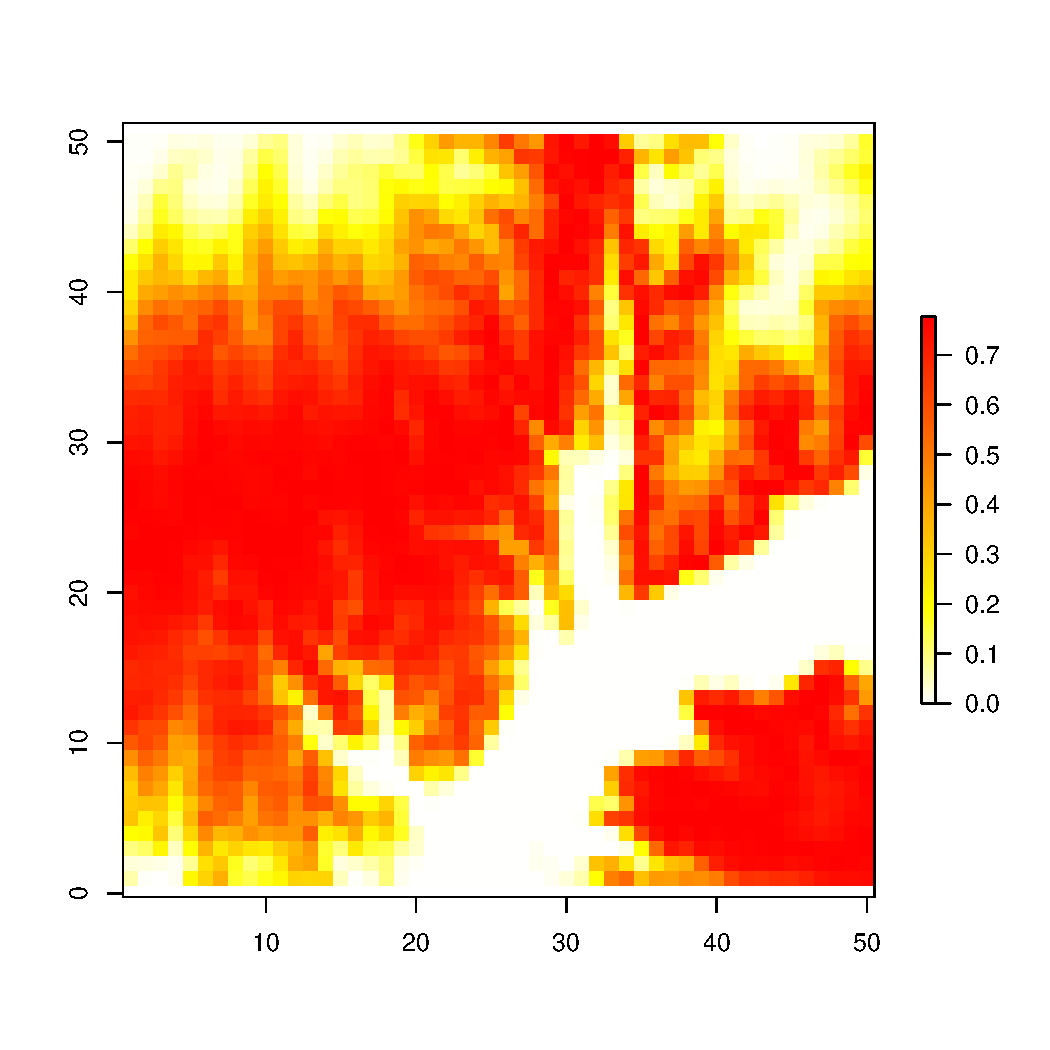
\includegraphics[width=8cm]{figures/theta-binomial.pdf} &
    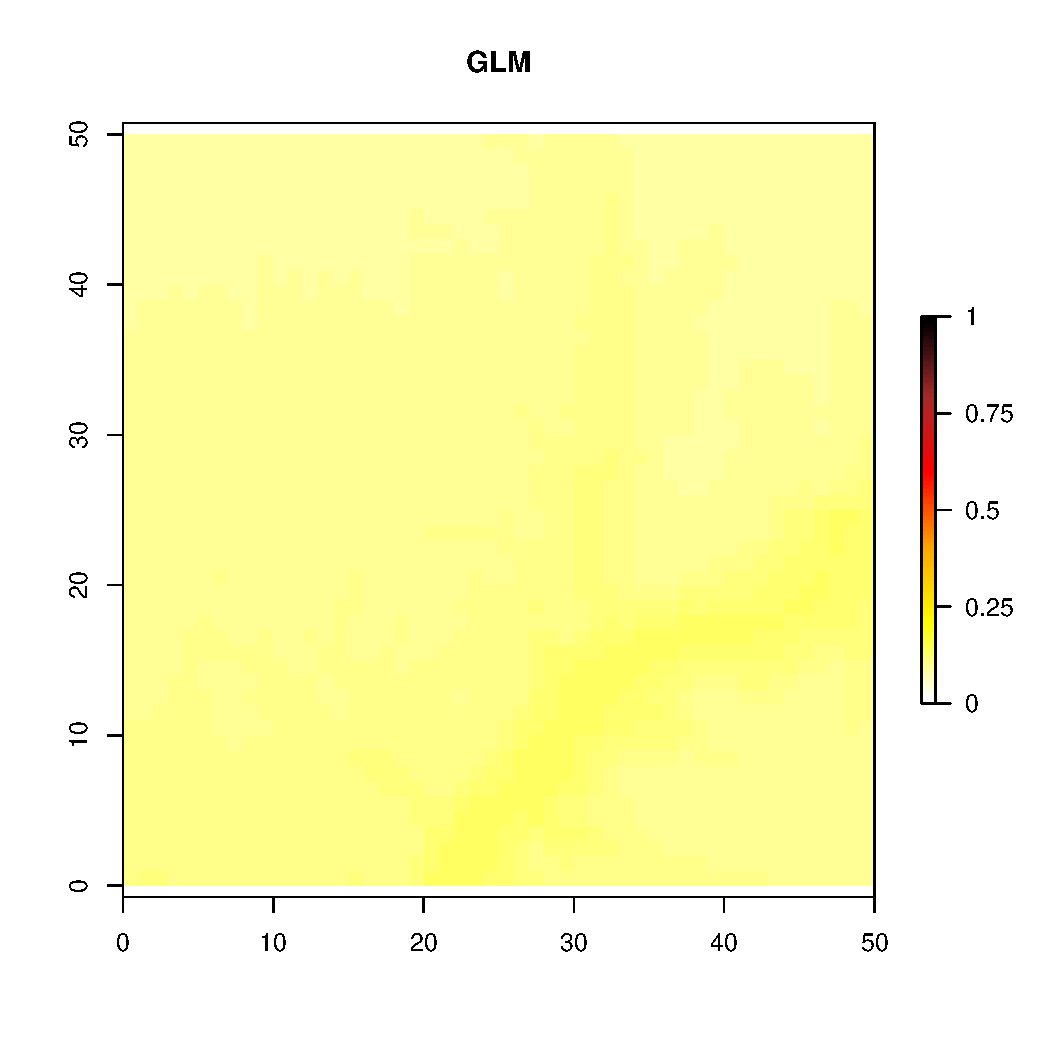
\includegraphics[width=8cm]{figures/predictions-siteocc-glm.pdf} \\
  \end{tabular}
  \centering 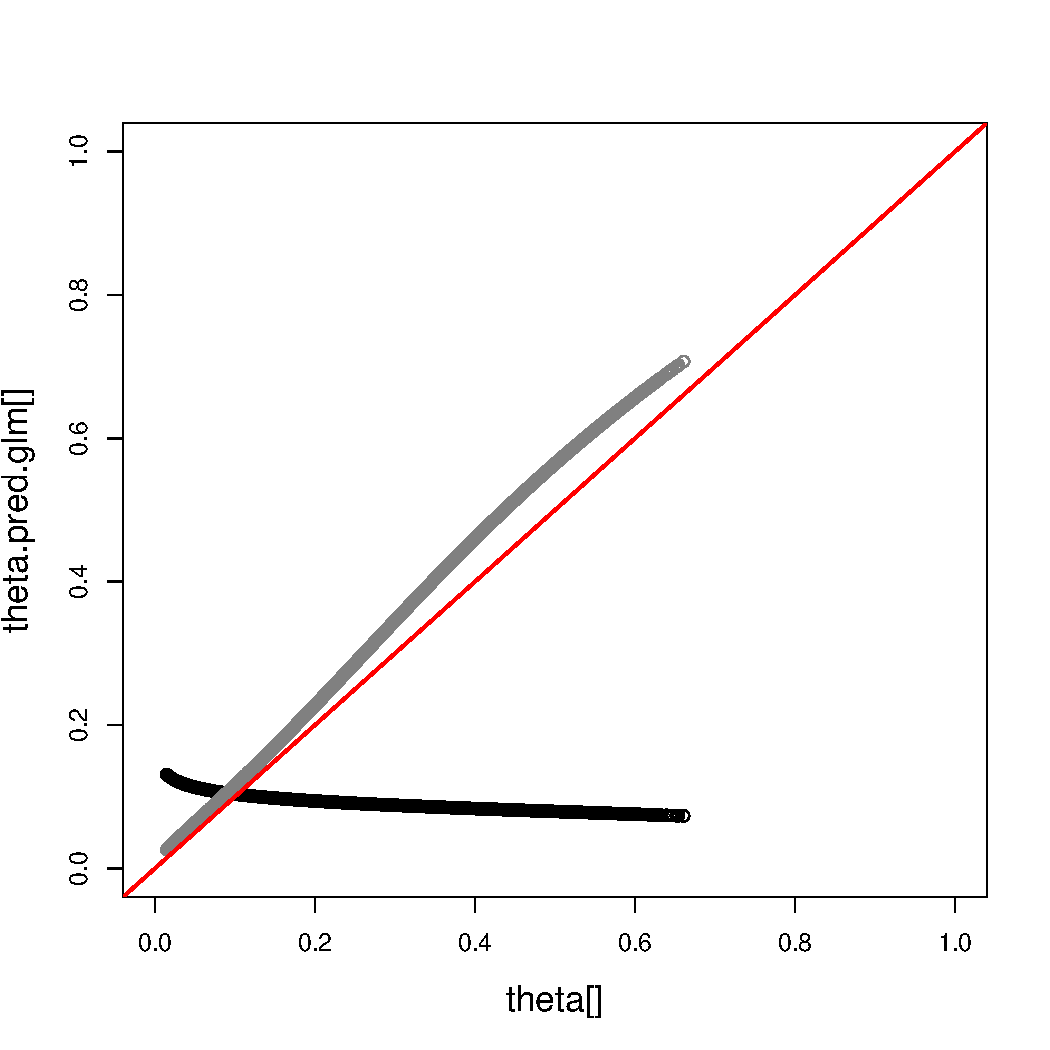
\includegraphics[width=8cm]{figures/pred-obs-siteocc-glm.pdf} \\
  
  \caption{\textbf{Comparing predicted probability of presence using glm with initial probabilities}}
  
  \label{fig:predictions-siteocc-glm}
  
\end{figure}



\subsection{Binomial iCAR model}

\subsection{Site-occupancy iCAR model}

\newpage

\section{Acknowledgements}

\newpage

\bibliographystyle{gcb}
\bibliography{/home/ghislain/Documents/Ghislain-CIRAD/Biblio/Biblio-These-GV}

\end{document}
